\documentclass[twoside]{book}

% Packages required by doxygen
\usepackage{fixltx2e}
\usepackage{calc}
\usepackage{doxygen}
\usepackage[export]{adjustbox} % also loads graphicx
\usepackage{graphicx}
\usepackage[utf8]{inputenc}
\usepackage{makeidx}
\usepackage{multicol}
\usepackage{multirow}
\PassOptionsToPackage{warn}{textcomp}
\usepackage{textcomp}
\usepackage[nointegrals]{wasysym}
\usepackage[table]{xcolor}

% Font selection
\usepackage[T1]{fontenc}
\usepackage[scaled=.90]{helvet}
\usepackage{courier}
\usepackage{amssymb}
\usepackage{sectsty}
\renewcommand{\familydefault}{\sfdefault}
\allsectionsfont{%
  \fontseries{bc}\selectfont%
  \color{darkgray}%
}
\renewcommand{\DoxyLabelFont}{%
  \fontseries{bc}\selectfont%
  \color{darkgray}%
}
\newcommand{\+}{\discretionary{\mbox{\scriptsize$\hookleftarrow$}}{}{}}

% Page & text layout
\usepackage{geometry}
\geometry{%
  a4paper,%
  top=2.5cm,%
  bottom=2.5cm,%
  left=2.5cm,%
  right=2.5cm%
}
\tolerance=750
\hfuzz=15pt
\hbadness=750
\setlength{\emergencystretch}{15pt}
\setlength{\parindent}{0cm}
\setlength{\parskip}{3ex plus 2ex minus 2ex}
\makeatletter
\renewcommand{\paragraph}{%
  \@startsection{paragraph}{4}{0ex}{-1.0ex}{1.0ex}{%
    \normalfont\normalsize\bfseries\SS@parafont%
  }%
}
\renewcommand{\subparagraph}{%
  \@startsection{subparagraph}{5}{0ex}{-1.0ex}{1.0ex}{%
    \normalfont\normalsize\bfseries\SS@subparafont%
  }%
}
\makeatother

% Headers & footers
\usepackage{fancyhdr}
\pagestyle{fancyplain}
\fancyhead[LE]{\fancyplain{}{\bfseries\thepage}}
\fancyhead[CE]{\fancyplain{}{}}
\fancyhead[RE]{\fancyplain{}{\bfseries\leftmark}}
\fancyhead[LO]{\fancyplain{}{\bfseries\rightmark}}
\fancyhead[CO]{\fancyplain{}{}}
\fancyhead[RO]{\fancyplain{}{\bfseries\thepage}}
\fancyfoot[LE]{\fancyplain{}{}}
\fancyfoot[CE]{\fancyplain{}{}}
\fancyfoot[RE]{\fancyplain{}{\bfseries\scriptsize Generated by Doxygen }}
\fancyfoot[LO]{\fancyplain{}{\bfseries\scriptsize Generated by Doxygen }}
\fancyfoot[CO]{\fancyplain{}{}}
\fancyfoot[RO]{\fancyplain{}{}}
\renewcommand{\footrulewidth}{0.4pt}
\renewcommand{\chaptermark}[1]{%
  \markboth{#1}{}%
}
\renewcommand{\sectionmark}[1]{%
  \markright{\thesection\ #1}%
}

% Indices & bibliography
\usepackage{natbib}
\usepackage[titles]{tocloft}
\setcounter{tocdepth}{3}
\setcounter{secnumdepth}{5}
\makeindex

% Hyperlinks (required, but should be loaded last)
\usepackage{ifpdf}
\ifpdf
  \usepackage[pdftex,pagebackref=true]{hyperref}
\else
  \usepackage[ps2pdf,pagebackref=true]{hyperref}
\fi
\hypersetup{%
  colorlinks=true,%
  linkcolor=blue,%
  citecolor=blue,%
  unicode%
}

% Custom commands
\newcommand{\clearemptydoublepage}{%
  \newpage{\pagestyle{empty}\cleardoublepage}%
}

\usepackage{caption}
\captionsetup{labelsep=space,justification=centering,font={bf},singlelinecheck=off,skip=4pt,position=top}

%===== C O N T E N T S =====

\begin{document}

% Titlepage & ToC
\hypersetup{pageanchor=false,
             bookmarksnumbered=true,
             pdfencoding=unicode
            }
\pagenumbering{alph}
\begin{titlepage}
\vspace*{7cm}
\begin{center}%
{\Large Magnificence 2 Chess }\\
\vspace*{1cm}
{\large Generated by Doxygen 1.8.13}\\
\end{center}
\end{titlepage}
\clearemptydoublepage
\pagenumbering{roman}
\tableofcontents
\clearemptydoublepage
\pagenumbering{arabic}
\hypersetup{pageanchor=true}

%--- Begin generated contents ---
\chapter{Hierarchical Index}
\section{Class Hierarchy}
This inheritance list is sorted roughly, but not completely, alphabetically\+:\begin{DoxyCompactList}
\item \contentsline{section}{Bit\+Board}{\pageref{classBitBoard}}{}
\item \contentsline{section}{Bit\+Board\+Base}{\pageref{structBitBoardBase}}{}
\item \contentsline{section}{Board\+Conversions}{\pageref{classBoardConversions}}{}
\item \contentsline{section}{Command\+Engine}{\pageref{classCommandEngine}}{}
\item \contentsline{section}{Engine}{\pageref{classEngine}}{}
\begin{DoxyCompactList}
\item \contentsline{section}{Engine\+Alpha\+Beta}{\pageref{classEngineAlphaBeta}}{}
\end{DoxyCompactList}
\item \contentsline{section}{Interface}{\pageref{classInterface}}{}
\item \contentsline{section}{Mail\+Board\+Base}{\pageref{structMailBoardBase}}{}
\item \contentsline{section}{Move}{\pageref{structMove}}{}
\item \contentsline{section}{String\+Arguments}{\pageref{structStringArguments}}{}
\item \contentsline{section}{String\+Helpers}{\pageref{classStringHelpers}}{}
\end{DoxyCompactList}

\chapter{Class Index}
\section{Class List}
Here are the classes, structs, unions and interfaces with brief descriptions\+:\begin{DoxyCompactList}
\item\contentsline{section}{\hyperlink{classBitBoard}{Bit\+Board} \\*A complete chess board implementation including make and unmake move }{\pageref{classBitBoard}}{}
\item\contentsline{section}{\hyperlink{structBitBoardBase}{Bit\+Board\+Base} \\*Wraps a vector to simplify move generation }{\pageref{structBitBoardBase}}{}
\item\contentsline{section}{\hyperlink{classBoardConversions}{Board\+Conversions} \\*This is a static helper class which is used for various Board state conversions and also other types of conversions which are needed }{\pageref{classBoardConversions}}{}
\item\contentsline{section}{\hyperlink{classCommandEngine}{Command\+Engine} \\*This class contains functions related to executing various commands sent from the \hyperlink{classInterface}{Interface} }{\pageref{classCommandEngine}}{}
\item\contentsline{section}{\hyperlink{classEngine}{Engine} \\*Base Chess \hyperlink{classEngine}{Engine} class, defines common variables and functions needed for children }{\pageref{classEngine}}{}
\item\contentsline{section}{\hyperlink{classEngineAlphaBeta}{Engine\+Alpha\+Beta} \\*Alpha Beta Chess \hyperlink{classEngine}{Engine} class. Inherits from base class \hyperlink{classEngine}{Engine} }{\pageref{classEngineAlphaBeta}}{}
\item\contentsline{section}{\hyperlink{classInterface}{Interface} \\*The main \hyperlink{classInterface}{Interface} class for the program. It controls the main command loop, reads input and executes commands by calling functions in \hyperlink{classCommandEngine}{Command\+Engine} }{\pageref{classInterface}}{}
\item\contentsline{section}{\hyperlink{structMailBoardBase}{Mail\+Board\+Base} \\*The basic data for a mail board }{\pageref{structMailBoardBase}}{}
\item\contentsline{section}{\hyperlink{structMove}{Move} \\*Chess move and stores the necessary data to unmake the move }{\pageref{structMove}}{}
\item\contentsline{section}{\hyperlink{structStringArguments}{String\+Arguments} \\*A class which is used to represents command inputs by splitting them up in parts for easier access }{\pageref{structStringArguments}}{}
\item\contentsline{section}{\hyperlink{classStringHelpers}{String\+Helpers} \\*A static helper class which is used for various common string tasks, such as string splitting }{\pageref{classStringHelpers}}{}
\end{DoxyCompactList}

\chapter{File Index}
\section{File List}
Here is a list of all documented files with brief descriptions\+:\begin{DoxyCompactList}
\item\contentsline{section}{src/\hyperlink{Main_8cpp}{Main.\+cpp} \\*Entry point for application }{\pageref{Main_8cpp}}{}
\item\contentsline{section}{src/\+Board/\hyperlink{BitBoard_8cpp}{Bit\+Board.\+cpp} }{\pageref{BitBoard_8cpp}}{}
\item\contentsline{section}{src/\+Board/\hyperlink{BitBoard_8h}{Bit\+Board.\+h} \\*Defines move and bitboard types }{\pageref{BitBoard_8h}}{}
\item\contentsline{section}{src/\+Board/\hyperlink{tests__bitboard_8h}{tests\+\_\+bitboard.\+h} }{\pageref{tests__bitboard_8h}}{}
\item\contentsline{section}{src/\+Board/{\bfseries type\+\_\+definitions.\+h} }{\pageref{type__definitions_8h}}{}
\item\contentsline{section}{src/\+Engine/\hyperlink{Engine_8h}{Engine.\+h} \\*Contains the \hyperlink{classEngine}{Engine} base class }{\pageref{Engine_8h}}{}
\item\contentsline{section}{src/\+Engine/\hyperlink{EngineAB_8h}{Engine\+A\+B.\+h} \\*Contains the class \hyperlink{classEngineAlphaBeta}{Engine\+Alpha\+Beta} }{\pageref{EngineAB_8h}}{}
\item\contentsline{section}{src/\+Interface/\hyperlink{BoardConversions_8h}{Board\+Conversions.\+h} \\*This file contains the static class \hyperlink{classBoardConversions}{Board\+Conversions} }{\pageref{BoardConversions_8h}}{}
\item\contentsline{section}{src/\+Interface/\hyperlink{CommandEngine_8h}{Command\+Engine.\+h} \\*This file contains the \hyperlink{classCommandEngine}{Command\+Engine} class }{\pageref{CommandEngine_8h}}{}
\item\contentsline{section}{src/\+Interface/\hyperlink{Interface_8h}{Interface.\+h} \\*This file contains the \hyperlink{classInterface}{Interface} class }{\pageref{Interface_8h}}{}
\item\contentsline{section}{src/\+Interface/\hyperlink{StringHelpers_8h}{String\+Helpers.\+h} \\*This file contains the static \hyperlink{classStringHelpers}{String\+Helpers} class and the \hyperlink{structStringArguments}{String\+Arguments} class }{\pageref{StringHelpers_8h}}{}
\end{DoxyCompactList}

\chapter{Class Documentation}
\hypertarget{classBitBoard}{}\section{Bit\+Board Class Reference}
\label{classBitBoard}\index{Bit\+Board@{Bit\+Board}}


A complete chess board implementation including make and unmake move.  




{\ttfamily \#include $<$Bit\+Board.\+h$>$}

\subsection*{Public Member Functions}
\begin{DoxyCompactItemize}
\item 
\mbox{\Hypertarget{classBitBoard_a16e5151e747beb21473ab790d60e4e36}\label{classBitBoard_a16e5151e747beb21473ab790d60e4e36}} 
\hyperlink{classBitBoard_a16e5151e747beb21473ab790d60e4e36}{Bit\+Board} ()
\begin{DoxyCompactList}\small\item\em Creates a new \hyperlink{classBitBoard}{Bit\+Board} in the startposition. \end{DoxyCompactList}\item 
\hyperlink{classBitBoard_aeaa1a16349090d393b00decbfe8eb6a6}{Bit\+Board} (const \hyperlink{classBitBoard}{Bit\+Board} \&original)
\begin{DoxyCompactList}\small\item\em Copies the given bitboard. \end{DoxyCompactList}\item 
\hyperlink{classBitBoard_aad0762329ff5f8455e177a6b58fbc64e}{Bit\+Board} (const std\+::string \&\hyperlink{classBitBoard_a5d5b2eea456fee2ce5246e1354fc4307}{fen\+\_\+string})
\begin{DoxyCompactList}\small\item\em Creates a board from a fen\+\_\+string. \end{DoxyCompactList}\item 
std\+::string \hyperlink{classBitBoard_a5d5b2eea456fee2ce5246e1354fc4307}{fen\+\_\+string} ()
\begin{DoxyCompactList}\small\item\em Creates and returns the fen string of the current position. \end{DoxyCompactList}\item 
const \hyperlink{structBitBoardBase}{Bit\+Board\+Base} \& \hyperlink{classBitBoard_ac8a51ff161d0271a81362c179465db69}{bitboard} ()
\begin{DoxyCompactList}\small\item\em Returns the bitboard representation of the board. \end{DoxyCompactList}\item 
const \hyperlink{structMailBoardBase}{Mail\+Board\+Base} \& \hyperlink{classBitBoard_a5397163febc786ddb7d9a324f37136da}{mailboard} ()
\begin{DoxyCompactList}\small\item\em Returns the mailboard representation of the board. \end{DoxyCompactList}\item 
void \hyperlink{classBitBoard_ad6a94224aa19bc86bbb14969d09a55e6}{make} (\hyperlink{structMove}{Move} move)
\begin{DoxyCompactList}\small\item\em Makes the given move. \end{DoxyCompactList}\item 
void \hyperlink{classBitBoard_ab81352f4aa143825a4763eba1947088c}{unmake} (\hyperlink{structMove}{Move} move)
\begin{DoxyCompactList}\small\item\em Unmakes the given move. \end{DoxyCompactList}\item 
\hyperlink{structMove}{Move} $\ast$ \hyperlink{classBitBoard_a1367722f40d889d95acdb6224cc34205}{move\+\_\+gen\+\_\+w} (\hyperlink{structMove}{Move} $\ast$move\+\_\+start\+\_\+buffer)
\begin{DoxyCompactList}\small\item\em Generates legal moves for white. \end{DoxyCompactList}\item 
\hyperlink{structMove}{Move} $\ast$ \hyperlink{classBitBoard_ae16917d3f752d11e5f689228d87bcf29}{move\+\_\+gen\+\_\+b} (\hyperlink{structMove}{Move} $\ast$move\+\_\+start\+\_\+buffer)
\begin{DoxyCompactList}\small\item\em Generates legal moves for black. \end{DoxyCompactList}\item 
\hyperlink{structMove}{Move} $\ast$ \hyperlink{classBitBoard_a5ce954a262cf51bee94d1508b9002464}{move\+\_\+gen} (\hyperlink{structMove}{Move} $\ast$move\+\_\+start\+\_\+buffer)
\begin{DoxyCompactList}\small\item\em Generates legal moves for the current player. \end{DoxyCompactList}\item 
bool \hyperlink{classBitBoard_a9a020e6d88fdedce0de800680abec2e7}{to\+\_\+move} ()
\begin{DoxyCompactList}\small\item\em returns the player to\+\_\+move, true for white, false for black \end{DoxyCompactList}\item 
u64 \hyperlink{classBitBoard_a0f58ac22e78e0045776e2ff0d6401d8e}{hash} ()
\begin{DoxyCompactList}\small\item\em Returns the zoobrist hash of the board. \end{DoxyCompactList}\end{DoxyCompactItemize}


\subsection{Detailed Description}
A complete chess board implementation including make and unmake move. 

\subsection{Constructor \& Destructor Documentation}
\mbox{\Hypertarget{classBitBoard_aeaa1a16349090d393b00decbfe8eb6a6}\label{classBitBoard_aeaa1a16349090d393b00decbfe8eb6a6}} 
\index{Bit\+Board@{Bit\+Board}!Bit\+Board@{Bit\+Board}}
\index{Bit\+Board@{Bit\+Board}!Bit\+Board@{Bit\+Board}}
\subsubsection{\texorpdfstring{Bit\+Board()}{BitBoard()}\hspace{0.1cm}{\footnotesize\ttfamily [1/2]}}
{\footnotesize\ttfamily Bit\+Board\+::\+Bit\+Board (\begin{DoxyParamCaption}\item[{const \hyperlink{classBitBoard}{Bit\+Board} \&}]{original }\end{DoxyParamCaption})\hspace{0.3cm}{\ttfamily [inline]}}



Copies the given bitboard. 


\begin{DoxyParams}{Parameters}
{\em original} & \\
\hline
\end{DoxyParams}
\mbox{\Hypertarget{classBitBoard_aad0762329ff5f8455e177a6b58fbc64e}\label{classBitBoard_aad0762329ff5f8455e177a6b58fbc64e}} 
\index{Bit\+Board@{Bit\+Board}!Bit\+Board@{Bit\+Board}}
\index{Bit\+Board@{Bit\+Board}!Bit\+Board@{Bit\+Board}}
\subsubsection{\texorpdfstring{Bit\+Board()}{BitBoard()}\hspace{0.1cm}{\footnotesize\ttfamily [2/2]}}
{\footnotesize\ttfamily Bit\+Board\+::\+Bit\+Board (\begin{DoxyParamCaption}\item[{const std\+::string \&}]{fen\+\_\+string }\end{DoxyParamCaption})\hspace{0.3cm}{\ttfamily [inline]}}



Creates a board from a fen\+\_\+string. 


\begin{DoxyParams}{Parameters}
{\em fen\+\_\+string} & \\
\hline
\end{DoxyParams}


\subsection{Member Function Documentation}
\mbox{\Hypertarget{classBitBoard_ac8a51ff161d0271a81362c179465db69}\label{classBitBoard_ac8a51ff161d0271a81362c179465db69}} 
\index{Bit\+Board@{Bit\+Board}!bitboard@{bitboard}}
\index{bitboard@{bitboard}!Bit\+Board@{Bit\+Board}}
\subsubsection{\texorpdfstring{bitboard()}{bitboard()}}
{\footnotesize\ttfamily const \hyperlink{structBitBoardBase}{Bit\+Board\+Base}\& Bit\+Board\+::bitboard (\begin{DoxyParamCaption}{ }\end{DoxyParamCaption})\hspace{0.3cm}{\ttfamily [inline]}}



Returns the bitboard representation of the board. 

\begin{DoxyReturn}{Returns}
const \hyperlink{structBitBoardBase}{Bit\+Board\+Base}\& 
\end{DoxyReturn}
\mbox{\Hypertarget{classBitBoard_a5d5b2eea456fee2ce5246e1354fc4307}\label{classBitBoard_a5d5b2eea456fee2ce5246e1354fc4307}} 
\index{Bit\+Board@{Bit\+Board}!fen\+\_\+string@{fen\+\_\+string}}
\index{fen\+\_\+string@{fen\+\_\+string}!Bit\+Board@{Bit\+Board}}
\subsubsection{\texorpdfstring{fen\+\_\+string()}{fen\_string()}}
{\footnotesize\ttfamily std\+::string Bit\+Board\+::fen\+\_\+string (\begin{DoxyParamCaption}{ }\end{DoxyParamCaption})\hspace{0.3cm}{\ttfamily [inline]}}



Creates and returns the fen string of the current position. 

\begin{DoxyReturn}{Returns}
std\+::string 
\end{DoxyReturn}
\mbox{\Hypertarget{classBitBoard_a0f58ac22e78e0045776e2ff0d6401d8e}\label{classBitBoard_a0f58ac22e78e0045776e2ff0d6401d8e}} 
\index{Bit\+Board@{Bit\+Board}!hash@{hash}}
\index{hash@{hash}!Bit\+Board@{Bit\+Board}}
\subsubsection{\texorpdfstring{hash()}{hash()}}
{\footnotesize\ttfamily u64 Bit\+Board\+::hash (\begin{DoxyParamCaption}{ }\end{DoxyParamCaption})\hspace{0.3cm}{\ttfamily [inline]}}



Returns the zoobrist hash of the board. 

\begin{DoxyReturn}{Returns}
u64 
\end{DoxyReturn}
\mbox{\Hypertarget{classBitBoard_a5397163febc786ddb7d9a324f37136da}\label{classBitBoard_a5397163febc786ddb7d9a324f37136da}} 
\index{Bit\+Board@{Bit\+Board}!mailboard@{mailboard}}
\index{mailboard@{mailboard}!Bit\+Board@{Bit\+Board}}
\subsubsection{\texorpdfstring{mailboard()}{mailboard()}}
{\footnotesize\ttfamily const \hyperlink{structMailBoardBase}{Mail\+Board\+Base}\& Bit\+Board\+::mailboard (\begin{DoxyParamCaption}{ }\end{DoxyParamCaption})\hspace{0.3cm}{\ttfamily [inline]}}



Returns the mailboard representation of the board. 

\begin{DoxyReturn}{Returns}
const \hyperlink{structMailBoardBase}{Mail\+Board\+Base}\& 
\end{DoxyReturn}
\mbox{\Hypertarget{classBitBoard_ad6a94224aa19bc86bbb14969d09a55e6}\label{classBitBoard_ad6a94224aa19bc86bbb14969d09a55e6}} 
\index{Bit\+Board@{Bit\+Board}!make@{make}}
\index{make@{make}!Bit\+Board@{Bit\+Board}}
\subsubsection{\texorpdfstring{make()}{make()}}
{\footnotesize\ttfamily void Bit\+Board\+::make (\begin{DoxyParamCaption}\item[{\hyperlink{structMove}{Move}}]{move }\end{DoxyParamCaption})\hspace{0.3cm}{\ttfamily [inline]}}



Makes the given move. 


\begin{DoxyParams}{Parameters}
{\em move} & \\
\hline
\end{DoxyParams}
\mbox{\Hypertarget{classBitBoard_a5ce954a262cf51bee94d1508b9002464}\label{classBitBoard_a5ce954a262cf51bee94d1508b9002464}} 
\index{Bit\+Board@{Bit\+Board}!move\+\_\+gen@{move\+\_\+gen}}
\index{move\+\_\+gen@{move\+\_\+gen}!Bit\+Board@{Bit\+Board}}
\subsubsection{\texorpdfstring{move\+\_\+gen()}{move\_gen()}}
{\footnotesize\ttfamily \hyperlink{structMove}{Move}$\ast$ Bit\+Board\+::move\+\_\+gen (\begin{DoxyParamCaption}\item[{\hyperlink{structMove}{Move} $\ast$}]{move\+\_\+start\+\_\+buffer }\end{DoxyParamCaption})\hspace{0.3cm}{\ttfamily [inline]}}



Generates legal moves for the current player. 


\begin{DoxyParams}{Parameters}
{\em move\+\_\+start\+\_\+buffer} & moves will be inserted with start here and new moves will be written to following adresses \\
\hline
\end{DoxyParams}
\begin{DoxyReturn}{Returns}
Move$\ast$ returns adress after the last move inserted 
\end{DoxyReturn}
\mbox{\Hypertarget{classBitBoard_ae16917d3f752d11e5f689228d87bcf29}\label{classBitBoard_ae16917d3f752d11e5f689228d87bcf29}} 
\index{Bit\+Board@{Bit\+Board}!move\+\_\+gen\+\_\+b@{move\+\_\+gen\+\_\+b}}
\index{move\+\_\+gen\+\_\+b@{move\+\_\+gen\+\_\+b}!Bit\+Board@{Bit\+Board}}
\subsubsection{\texorpdfstring{move\+\_\+gen\+\_\+b()}{move\_gen\_b()}}
{\footnotesize\ttfamily \hyperlink{structMove}{Move}$\ast$ Bit\+Board\+::move\+\_\+gen\+\_\+b (\begin{DoxyParamCaption}\item[{\hyperlink{structMove}{Move} $\ast$}]{move\+\_\+start\+\_\+buffer }\end{DoxyParamCaption})\hspace{0.3cm}{\ttfamily [inline]}}



Generates legal moves for black. 


\begin{DoxyParams}{Parameters}
{\em move\+\_\+start\+\_\+buffer} & moves will be inserted with start here and new moves will be written to following adresses \\
\hline
\end{DoxyParams}
\begin{DoxyReturn}{Returns}
Move$\ast$ returns adress after the last move inserted 
\end{DoxyReturn}
\mbox{\Hypertarget{classBitBoard_a1367722f40d889d95acdb6224cc34205}\label{classBitBoard_a1367722f40d889d95acdb6224cc34205}} 
\index{Bit\+Board@{Bit\+Board}!move\+\_\+gen\+\_\+w@{move\+\_\+gen\+\_\+w}}
\index{move\+\_\+gen\+\_\+w@{move\+\_\+gen\+\_\+w}!Bit\+Board@{Bit\+Board}}
\subsubsection{\texorpdfstring{move\+\_\+gen\+\_\+w()}{move\_gen\_w()}}
{\footnotesize\ttfamily \hyperlink{structMove}{Move}$\ast$ Bit\+Board\+::move\+\_\+gen\+\_\+w (\begin{DoxyParamCaption}\item[{\hyperlink{structMove}{Move} $\ast$}]{move\+\_\+start\+\_\+buffer }\end{DoxyParamCaption})\hspace{0.3cm}{\ttfamily [inline]}}



Generates legal moves for white. 


\begin{DoxyParams}{Parameters}
{\em move\+\_\+start\+\_\+buffer} & moves will be inserted with start here and new moves will be written to following adresses \\
\hline
\end{DoxyParams}
\begin{DoxyReturn}{Returns}
Move$\ast$ returns adress after the last move inserted 
\end{DoxyReturn}
\mbox{\Hypertarget{classBitBoard_a9a020e6d88fdedce0de800680abec2e7}\label{classBitBoard_a9a020e6d88fdedce0de800680abec2e7}} 
\index{Bit\+Board@{Bit\+Board}!to\+\_\+move@{to\+\_\+move}}
\index{to\+\_\+move@{to\+\_\+move}!Bit\+Board@{Bit\+Board}}
\subsubsection{\texorpdfstring{to\+\_\+move()}{to\_move()}}
{\footnotesize\ttfamily bool Bit\+Board\+::to\+\_\+move (\begin{DoxyParamCaption}{ }\end{DoxyParamCaption})\hspace{0.3cm}{\ttfamily [inline]}}



returns the player to\+\_\+move, true for white, false for black 

\begin{DoxyReturn}{Returns}
Bool 
\end{DoxyReturn}
\mbox{\Hypertarget{classBitBoard_ab81352f4aa143825a4763eba1947088c}\label{classBitBoard_ab81352f4aa143825a4763eba1947088c}} 
\index{Bit\+Board@{Bit\+Board}!unmake@{unmake}}
\index{unmake@{unmake}!Bit\+Board@{Bit\+Board}}
\subsubsection{\texorpdfstring{unmake()}{unmake()}}
{\footnotesize\ttfamily void Bit\+Board\+::unmake (\begin{DoxyParamCaption}\item[{\hyperlink{structMove}{Move}}]{move }\end{DoxyParamCaption})\hspace{0.3cm}{\ttfamily [inline]}}



Unmakes the given move. 


\begin{DoxyParams}{Parameters}
{\em move} & \\
\hline
\end{DoxyParams}


The documentation for this class was generated from the following file\+:\begin{DoxyCompactItemize}
\item 
src/\+Board/\hyperlink{BitBoard_8h}{Bit\+Board.\+h}\end{DoxyCompactItemize}

\hypertarget{structBitBoardBase}{}\section{Bit\+Board\+Base Struct Reference}
\label{structBitBoardBase}\index{Bit\+Board\+Base@{Bit\+Board\+Base}}


Wraps a vector to simplify move generation.  




{\ttfamily \#include $<$Bit\+Board.\+h$>$}

\subsection*{Public Attributes}
\begin{DoxyCompactItemize}
\item 
\mbox{\Hypertarget{structBitBoardBase_a1fd8c1b15e2e329e89b932fb5c3c4811}\label{structBitBoardBase_a1fd8c1b15e2e329e89b932fb5c3c4811}} 
u64 \hyperlink{structBitBoardBase_a1fd8c1b15e2e329e89b932fb5c3c4811}{pieces} \mbox{[}13\mbox{]}
\begin{DoxyCompactList}\small\item\em 0\+: empty, 1\+: w\+Pawn, 2\+: w\+Knight, 3\+:w\+Bishop, 4\+: w\+Rook, 5\+: w\+Queen, 6\+: w\+King, 7\+: b\+Pawn, 8\+: b\+Knight, 9\+: b\+Bishop, 10\+: b\+Rook, 11\+: b\+Queen, 12\+: b\+King \end{DoxyCompactList}\end{DoxyCompactItemize}


\subsection{Detailed Description}
Wraps a vector to simplify move generation. 

The basic data for a bitboard 

The documentation for this struct was generated from the following file\+:\begin{DoxyCompactItemize}
\item 
src/\+Board/\hyperlink{BitBoard_8h}{Bit\+Board.\+h}\end{DoxyCompactItemize}

\hypertarget{classBoardConversions}{}\section{Board\+Conversions Class Reference}
\label{classBoardConversions}\index{Board\+Conversions@{Board\+Conversions}}


This is a static helper class which is used for various Board state conversions and also other types of conversions which are needed.  




{\ttfamily \#include $<$Board\+Conversions.\+h$>$}

\subsection*{Static Public Member Functions}
\begin{DoxyCompactItemize}
\item 
\mbox{\Hypertarget{classBoardConversions_aef2786eee5b3d96aa23aa9ca2b38f693}\label{classBoardConversions_aef2786eee5b3d96aa23aa9ca2b38f693}} 
static std\+::string \hyperlink{classBoardConversions_aef2786eee5b3d96aa23aa9ca2b38f693}{bb\+To\+Display\+String} (\hyperlink{classBitBoard}{Bit\+Board} \&board)
\begin{DoxyCompactList}\small\item\em This function converts a Bitboard class to a prettified string notation used for testing. \end{DoxyCompactList}\item 
\mbox{\Hypertarget{classBoardConversions_a6fb57142a68ffbc456ad518778e299e3}\label{classBoardConversions_a6fb57142a68ffbc456ad518778e299e3}} 
static std\+::string \hyperlink{classBoardConversions_a6fb57142a68ffbc456ad518778e299e3}{bb\+To\+Fen\+String} (\hyperlink{classBitBoard}{Bit\+Board} \&board)
\begin{DoxyCompactList}\small\item\em This function converts a Bitboard class to the F\+EN standard notation (string) F\+EN example (starting position)\+: rnbqkbnr/pppppppp/8/8/8/8/\+P\+P\+P\+P\+P\+P\+P\+P/\+R\+N\+B\+Q\+K\+B\+NR w K\+Qkq -\/ 0 1. \end{DoxyCompactList}\item 
\mbox{\Hypertarget{classBoardConversions_ae16a4fe316818ea8a006d7050f37701c}\label{classBoardConversions_ae16a4fe316818ea8a006d7050f37701c}} 
static std\+::string \hyperlink{classBoardConversions_ae16a4fe316818ea8a006d7050f37701c}{move\+To\+Algebaric\+Move} (\hyperlink{structMove}{Move} \&move)
\begin{DoxyCompactList}\small\item\em This function converts a \hyperlink{structMove}{Move} struct to Algebraic \hyperlink{structMove}{Move} Notation (string, ex \textquotesingle{}a2a3\textquotesingle{}) \end{DoxyCompactList}\item 
\mbox{\Hypertarget{classBoardConversions_a1db0f37732123cb9d104d83c398e51b0}\label{classBoardConversions_a1db0f37732123cb9d104d83c398e51b0}} 
static \hyperlink{structMove}{Move} \hyperlink{classBoardConversions_a1db0f37732123cb9d104d83c398e51b0}{algebraic\+Move\+To\+Move} (std\+::string alg\+Move)
\begin{DoxyCompactList}\small\item\em This function converts a string of Algebraic \hyperlink{structMove}{Move} Notation (ex \textquotesingle{}a2a3\textquotesingle{}) to a \hyperlink{structMove}{Move} Struct. \end{DoxyCompactList}\end{DoxyCompactItemize}


\subsection{Detailed Description}
This is a static helper class which is used for various Board state conversions and also other types of conversions which are needed. 

Examples are the Bitboard class to F\+EN strings (a standardized of representing a chess board with a string), the \hyperlink{structMove}{Move} struct to algebraic string form etc. 

The documentation for this class was generated from the following files\+:\begin{DoxyCompactItemize}
\item 
src/\+Interface/\hyperlink{BoardConversions_8h}{Board\+Conversions.\+h}\item 
src/\+Interface/Board\+Conversions.\+cpp\end{DoxyCompactItemize}

\hypertarget{classCommandEngine}{}\section{Command\+Engine Class Reference}
\label{classCommandEngine}\index{Command\+Engine@{Command\+Engine}}


This class contains functions related to executing various commands sent from the \hyperlink{classInterface}{Interface}.  




{\ttfamily \#include $<$Command\+Engine.\+h$>$}

\subsection*{Public Types}
\begin{DoxyCompactItemize}
\item 
\mbox{\Hypertarget{classCommandEngine_ad9c039b48df85947ae760da43e7cedb9}\label{classCommandEngine_ad9c039b48df85947ae760da43e7cedb9}} 
enum {\bfseries Interface\+Mode} \{ {\bfseries T\+E\+S\+T\+I\+NG}, 
{\bfseries U\+CI}
 \}
\item 
\mbox{\Hypertarget{classCommandEngine_aac6dff88a64e7e98e0500558bf15afa8}\label{classCommandEngine_aac6dff88a64e7e98e0500558bf15afa8}} 
typedef void(Command\+Engine\+::$\ast$ {\bfseries Command\+Function}) (\hyperlink{structStringArguments}{String\+Arguments} \&)
\end{DoxyCompactItemize}
\subsection*{Public Member Functions}
\begin{DoxyCompactItemize}
\item 
\mbox{\Hypertarget{classCommandEngine_a76c27f3933326c261d709618d7f996c7}\label{classCommandEngine_a76c27f3933326c261d709618d7f996c7}} 
void \hyperlink{classCommandEngine_a76c27f3933326c261d709618d7f996c7}{cmd\+Display} (\hyperlink{structStringArguments}{String\+Arguments} \&arguments)
\begin{DoxyCompactList}\small\item\em display. Display the board prettily in the console \end{DoxyCompactList}\item 
\mbox{\Hypertarget{classCommandEngine_a1ce6ddfd0eb350cfdde728458329f67d}\label{classCommandEngine_a1ce6ddfd0eb350cfdde728458329f67d}} 
void \hyperlink{classCommandEngine_a1ce6ddfd0eb350cfdde728458329f67d}{cmd\+Help} (\hyperlink{structStringArguments}{String\+Arguments} \&arguments)
\begin{DoxyCompactList}\small\item\em cmd\+: help. Display a list of commands \end{DoxyCompactList}\item 
\mbox{\Hypertarget{classCommandEngine_ad82f0bf1cb89f7f43288ce379f97be04}\label{classCommandEngine_ad82f0bf1cb89f7f43288ce379f97be04}} 
void \hyperlink{classCommandEngine_ad82f0bf1cb89f7f43288ce379f97be04}{cmd\+Quit} (\hyperlink{structStringArguments}{String\+Arguments} \&arguments)
\begin{DoxyCompactList}\small\item\em cmd\+: quit. Exit the program \end{DoxyCompactList}\item 
\mbox{\Hypertarget{classCommandEngine_ac70f9158e992aa4d7567fa2fe47b09e7}\label{classCommandEngine_ac70f9158e992aa4d7567fa2fe47b09e7}} 
void \hyperlink{classCommandEngine_ac70f9158e992aa4d7567fa2fe47b09e7}{cmd\+Perft} (\hyperlink{structStringArguments}{String\+Arguments} \&arguments)
\begin{DoxyCompactList}\small\item\em cmd\+: perft $<$depth$>$. Does a $<$depth$>$ deep counting of leaf nodes in the legal moves tree \end{DoxyCompactList}\item 
\mbox{\Hypertarget{classCommandEngine_ad6f3a8998e456a4efa626e32219e1406}\label{classCommandEngine_ad6f3a8998e456a4efa626e32219e1406}} 
void \hyperlink{classCommandEngine_ad6f3a8998e456a4efa626e32219e1406}{cmd\+Fen} (\hyperlink{structStringArguments}{String\+Arguments} \&arguments)
\begin{DoxyCompactList}\small\item\em cmd\+: fen. Outputs the board as a fen string \end{DoxyCompactList}\item 
\mbox{\Hypertarget{classCommandEngine_a3c3140b31ac623d4b84611dfe954f3f0}\label{classCommandEngine_a3c3140b31ac623d4b84611dfe954f3f0}} 
void {\bfseries cmd\+Self\+Play} (\hyperlink{structStringArguments}{String\+Arguments} \&arguments)
\item 
\mbox{\Hypertarget{classCommandEngine_a1b1dfc2c6c5f0a161b68639b44798030}\label{classCommandEngine_a1b1dfc2c6c5f0a161b68639b44798030}} 
void \hyperlink{classCommandEngine_a1b1dfc2c6c5f0a161b68639b44798030}{cmd\+Divide} (\hyperlink{structStringArguments}{String\+Arguments} \&arguments)
\begin{DoxyCompactList}\small\item\em \+: cmd divide. Perft score per each legal move of current position. Useful for debugging movegen \end{DoxyCompactList}\item 
\mbox{\Hypertarget{classCommandEngine_ac508155eaada08bbab04d6644339fa87}\label{classCommandEngine_ac508155eaada08bbab04d6644339fa87}} 
void \hyperlink{classCommandEngine_ac508155eaada08bbab04d6644339fa87}{cmd\+Move} (\hyperlink{structStringArguments}{String\+Arguments} \&arguments)
\begin{DoxyCompactList}\small\item\em \+: cmd move $<$move$>$. \hyperlink{structMove}{Move} an algebraic move. \end{DoxyCompactList}\item 
\mbox{\Hypertarget{classCommandEngine_a2eec96165224a39d01c5c8803aec9dc6}\label{classCommandEngine_a2eec96165224a39d01c5c8803aec9dc6}} 
void \hyperlink{classCommandEngine_a2eec96165224a39d01c5c8803aec9dc6}{cmd\+Legal\+Moves} (\hyperlink{structStringArguments}{String\+Arguments} \&arguments)
\begin{DoxyCompactList}\small\item\em \+: cmd moves. List the legal moves \end{DoxyCompactList}\item 
\mbox{\Hypertarget{classCommandEngine_a68d00effca283abfb561aacbad1977c9}\label{classCommandEngine_a68d00effca283abfb561aacbad1977c9}} 
void \hyperlink{classCommandEngine_a68d00effca283abfb561aacbad1977c9}{cmd\+Go} (\hyperlink{structStringArguments}{String\+Arguments} \&arguments)
\begin{DoxyCompactList}\small\item\em cmd\+: go. Starts searching in the engine on a separate thread Received command in this format\+: \char`\"{}go wtime 300000 btime 300000 winc 0 binc 0\char`\"{} Also allowed\+: \char`\"{}go $<$maxdepth$>$\char`\"{} Output format\+: \char`\"{}bestmove h7h5\char`\"{} \end{DoxyCompactList}\item 
\mbox{\Hypertarget{classCommandEngine_a60549918b43f3e5a3a9c046dcd3b74bb}\label{classCommandEngine_a60549918b43f3e5a3a9c046dcd3b74bb}} 
void \hyperlink{classCommandEngine_a60549918b43f3e5a3a9c046dcd3b74bb}{cmd\+U\+CI} (\hyperlink{structStringArguments}{String\+Arguments} \&arguments)
\begin{DoxyCompactList}\small\item\em cmd\+: uci. Enter U\+CI mode \end{DoxyCompactList}\item 
\mbox{\Hypertarget{classCommandEngine_a0a3ff3017005a6cbd5f347def93df769}\label{classCommandEngine_a0a3ff3017005a6cbd5f347def93df769}} 
void {\bfseries cmd\+Position} (\hyperlink{structStringArguments}{String\+Arguments} \&arguments)
\item 
\mbox{\Hypertarget{classCommandEngine_a2db9a6317c944a436cc57d686b82e317}\label{classCommandEngine_a2db9a6317c944a436cc57d686b82e317}} 
void \hyperlink{classCommandEngine_a2db9a6317c944a436cc57d686b82e317}{cmd\+Set\+Board} (\hyperlink{structStringArguments}{String\+Arguments} \&arguments)
\begin{DoxyCompactList}\small\item\em cmd\+: setboard. Set the board to a fen string \end{DoxyCompactList}\item 
\mbox{\Hypertarget{classCommandEngine_a93c928fa42978803696d94d6e2ab4e40}\label{classCommandEngine_a93c928fa42978803696d94d6e2ab4e40}} 
void \hyperlink{classCommandEngine_a93c928fa42978803696d94d6e2ab4e40}{cmd\+Stop} (\hyperlink{structStringArguments}{String\+Arguments} \&arguments)
\begin{DoxyCompactList}\small\item\em cmd\+: stop. Stop the engine search \end{DoxyCompactList}\item 
\mbox{\Hypertarget{classCommandEngine_ad9bf2d5479c8d9c15713f51101676860}\label{classCommandEngine_ad9bf2d5479c8d9c15713f51101676860}} 
void \hyperlink{classCommandEngine_ad9bf2d5479c8d9c15713f51101676860}{cmd\+Is\+Ready} (\hyperlink{structStringArguments}{String\+Arguments} \&arguments)
\begin{DoxyCompactList}\small\item\em cmd\+: isready. Replies with readyok if engine is ready for new commands \end{DoxyCompactList}\item 
\mbox{\Hypertarget{classCommandEngine_a6c4da85ce98949d0b12abe5913397a65}\label{classCommandEngine_a6c4da85ce98949d0b12abe5913397a65}} 
bool \hyperlink{classCommandEngine_a6c4da85ce98949d0b12abe5913397a65}{are\+Arguments\+Correcly\+Formatted} (\hyperlink{structStringArguments}{String\+Arguments} \&arguments, int size)
\begin{DoxyCompactList}\small\item\em Checks that a command is correctly formatted by checking the number of arguments equals the given number. \end{DoxyCompactList}\item 
\mbox{\Hypertarget{classCommandEngine_a7a8ea24982fe014a3d0518fabb9fba5c}\label{classCommandEngine_a7a8ea24982fe014a3d0518fabb9fba5c}} 
void \hyperlink{classCommandEngine_a7a8ea24982fe014a3d0518fabb9fba5c}{error\+Message} (std\+::string message)
\begin{DoxyCompactList}\small\item\em Sends an error message related to a command. It is only sent in Testing mode, U\+CI does not accept other output like this. \end{DoxyCompactList}\end{DoxyCompactItemize}
\subsection*{Public Attributes}
\begin{DoxyCompactItemize}
\item 
\mbox{\Hypertarget{classCommandEngine_ab046274e8d4cf871fd392aafd7e37214}\label{classCommandEngine_ab046274e8d4cf871fd392aafd7e37214}} 
bool {\bfseries exit} = false
\item 
\mbox{\Hypertarget{classCommandEngine_aa7b5bb7e6195276e5bc77d5335fc749f}\label{classCommandEngine_aa7b5bb7e6195276e5bc77d5335fc749f}} 
Interface\+Mode {\bfseries interface\+Mode} = T\+E\+S\+T\+I\+NG
\item 
\mbox{\Hypertarget{classCommandEngine_a6d7699fde08924a6dc99516948d1c7ca}\label{classCommandEngine_a6d7699fde08924a6dc99516948d1c7ca}} 
std\+::atomic$<$ bool $>$ {\bfseries currently\+Searching} \{false\}
\end{DoxyCompactItemize}


\subsection{Detailed Description}
This class contains functions related to executing various commands sent from the \hyperlink{classInterface}{Interface}. 

The command functions in this class are used by the \hyperlink{classInterface}{Interface} through function pointers. All the command functions recieve a \hyperlink{structStringArguments}{String\+Arguments} struct which contain information regarding the input that the interface recieved to trigger this function, ie flags and arguments and such. The \hyperlink{classCommandEngine}{Command\+Engine} has ownership of the main chess \hyperlink{classEngine}{Engine} as well as a side \hyperlink{classEngine}{Engine} (which is used for selfplay testing) It also has control of a separate thread which is used to initiate searching in the main engine. This is needed as the U\+CI standard requires responsiveness during searching. 

The documentation for this class was generated from the following files\+:\begin{DoxyCompactItemize}
\item 
src/\+Interface/\hyperlink{CommandEngine_8h}{Command\+Engine.\+h}\item 
src/\+Interface/Command\+Engine.\+cpp\end{DoxyCompactItemize}

\hypertarget{classEngine}{}\section{Engine Class Reference}
\label{classEngine}\index{Engine@{Engine}}


Base Chess \hyperlink{classEngine}{Engine} class, defines common variables and functions needed for children.  




{\ttfamily \#include $<$Engine.\+h$>$}



Inheritance diagram for Engine\+:\nopagebreak
\begin{figure}[H]
\begin{center}
\leavevmode
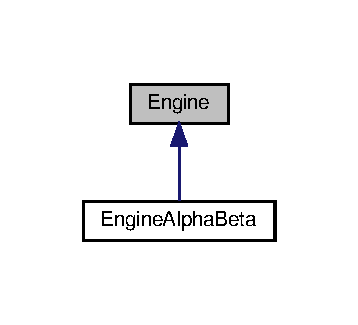
\includegraphics[width=172pt]{classEngine__inherit__graph}
\end{center}
\end{figure}


Collaboration diagram for Engine\+:\nopagebreak
\begin{figure}[H]
\begin{center}
\leavevmode
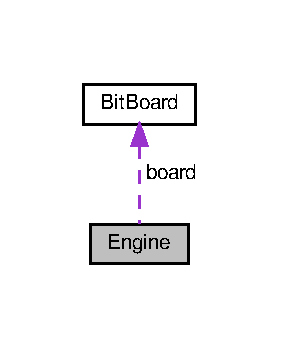
\includegraphics[width=135pt]{classEngine__coll__graph}
\end{center}
\end{figure}
\subsection*{Public Member Functions}
\begin{DoxyCompactItemize}
\item 
\mbox{\Hypertarget{classEngine_a28c4c89b8c2f42e2d88d3c5d315b5d3e}\label{classEngine_a28c4c89b8c2f42e2d88d3c5d315b5d3e}} 
virtual void {\bfseries search} ()
\end{DoxyCompactItemize}
\subsection*{Public Attributes}
\begin{DoxyCompactItemize}
\item 
\mbox{\Hypertarget{classEngine_a1e66131e0b0661930088212610583ad7}\label{classEngine_a1e66131e0b0661930088212610583ad7}} 
int {\bfseries max\+Depth} = 0
\item 
\mbox{\Hypertarget{classEngine_a06bbc29b6477258954a6108f08e80bc2}\label{classEngine_a06bbc29b6477258954a6108f08e80bc2}} 
bool {\bfseries color} = true
\item 
\mbox{\Hypertarget{classEngine_aae0b47bca9ae3bd3f2fefd12ab2b2455}\label{classEngine_aae0b47bca9ae3bd3f2fefd12ab2b2455}} 
\hyperlink{classBitBoard}{Bit\+Board} {\bfseries board}
\item 
\mbox{\Hypertarget{classEngine_a31fde0cdd9928f7662dab2cf88b2fb43}\label{classEngine_a31fde0cdd9928f7662dab2cf88b2fb43}} 
bool {\bfseries stop\+Searching} = false
\item 
\mbox{\Hypertarget{classEngine_a72f5b4117314a68b938383915ad3ef51}\label{classEngine_a72f5b4117314a68b938383915ad3ef51}} 
std\+::vector$<$ u32 $>$ {\bfseries principal\+Variation}
\end{DoxyCompactItemize}


\subsection{Detailed Description}
Base Chess \hyperlink{classEngine}{Engine} class, defines common variables and functions needed for children. 

The documentation for this class was generated from the following file\+:\begin{DoxyCompactItemize}
\item 
src/\+Engine/\hyperlink{Engine_8h}{Engine.\+h}\end{DoxyCompactItemize}

\hypertarget{classEngineAlphaBeta}{}\section{Engine\+Alpha\+Beta Class Reference}
\label{classEngineAlphaBeta}\index{Engine\+Alpha\+Beta@{Engine\+Alpha\+Beta}}


Alpha Beta Chess \hyperlink{classEngine}{Engine} class. Inherits from base class \hyperlink{classEngine}{Engine}.  




{\ttfamily \#include $<$Engine\+A\+B.\+h$>$}



Inheritance diagram for Engine\+Alpha\+Beta\+:\nopagebreak
\begin{figure}[H]
\begin{center}
\leavevmode
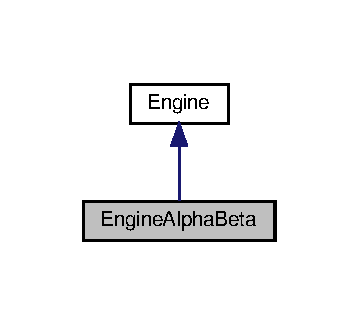
\includegraphics[width=172pt]{classEngineAlphaBeta__inherit__graph}
\end{center}
\end{figure}


Collaboration diagram for Engine\+Alpha\+Beta\+:\nopagebreak
\begin{figure}[H]
\begin{center}
\leavevmode
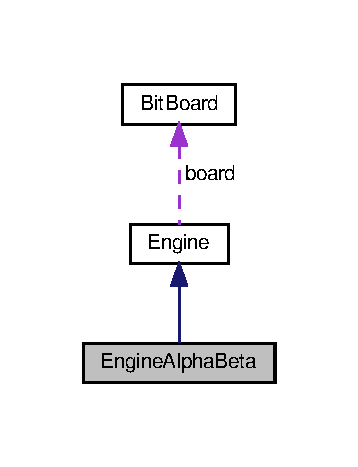
\includegraphics[width=172pt]{classEngineAlphaBeta__coll__graph}
\end{center}
\end{figure}
\subsection*{Public Member Functions}
\begin{DoxyCompactItemize}
\item 
\mbox{\Hypertarget{classEngineAlphaBeta_afea6d4b88e7fe762f31208645bdbd203}\label{classEngineAlphaBeta_afea6d4b88e7fe762f31208645bdbd203}} 
void \hyperlink{classEngineAlphaBeta_afea6d4b88e7fe762f31208645bdbd203}{search} () override
\begin{DoxyCompactList}\small\item\em Alpha Beta prototype search. \end{DoxyCompactList}\end{DoxyCompactItemize}
\subsection*{Public Attributes}
\begin{DoxyCompactItemize}
\item 
\mbox{\Hypertarget{classEngineAlphaBeta_a40e006a5eb4f51f468914de7b1f33747}\label{classEngineAlphaBeta_a40e006a5eb4f51f468914de7b1f33747}} 
int {\bfseries test} = 15
\end{DoxyCompactItemize}


\subsection{Detailed Description}
Alpha Beta Chess \hyperlink{classEngine}{Engine} class. Inherits from base class \hyperlink{classEngine}{Engine}. 

The documentation for this class was generated from the following files\+:\begin{DoxyCompactItemize}
\item 
src/\+Engine/\hyperlink{EngineAB_8h}{Engine\+A\+B.\+h}\item 
src/\+Engine/Engine\+A\+B.\+cpp\end{DoxyCompactItemize}

\hypertarget{classInterface}{}\section{Interface Class Reference}
\label{classInterface}\index{Interface@{Interface}}


The main \hyperlink{classInterface}{Interface} class for the program. It controls the main command loop, reads input and executes commands by calling functions in \hyperlink{classCommandEngine}{Command\+Engine}.  




{\ttfamily \#include $<$Interface.\+h$>$}



Collaboration diagram for Interface\+:\nopagebreak
\begin{figure}[H]
\begin{center}
\leavevmode
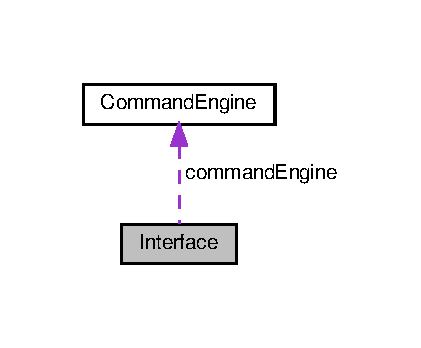
\includegraphics[width=202pt]{classInterface__coll__graph}
\end{center}
\end{figure}
\subsection*{Public Member Functions}
\begin{DoxyCompactItemize}
\item 
\mbox{\Hypertarget{classInterface_a90eb0675e0534a93b6486065da5168a9}\label{classInterface_a90eb0675e0534a93b6486065da5168a9}} 
void {\bfseries setup} ()
\item 
\mbox{\Hypertarget{classInterface_a090a950300a463d91f8f361d3b333906}\label{classInterface_a090a950300a463d91f8f361d3b333906}} 
void {\bfseries run} ()
\end{DoxyCompactItemize}
\subsection*{Public Attributes}
\begin{DoxyCompactItemize}
\item 
\mbox{\Hypertarget{classInterface_a5a2c86a63a352460d715f580568aabad}\label{classInterface_a5a2c86a63a352460d715f580568aabad}} 
\hyperlink{classCommandEngine}{Command\+Engine} {\bfseries command\+Engine}
\end{DoxyCompactItemize}


\subsection{Detailed Description}
The main \hyperlink{classInterface}{Interface} class for the program. It controls the main command loop, reads input and executes commands by calling functions in \hyperlink{classCommandEngine}{Command\+Engine}. 

The documentation for this class was generated from the following files\+:\begin{DoxyCompactItemize}
\item 
src/\+Interface/\hyperlink{Interface_8h}{Interface.\+h}\item 
src/\+Interface/Interface.\+cpp\end{DoxyCompactItemize}

\hypertarget{structMailBoardBase}{}\section{Mail\+Board\+Base Struct Reference}
\label{structMailBoardBase}\index{Mail\+Board\+Base@{Mail\+Board\+Base}}


The basic data for a mail board.  




{\ttfamily \#include $<$Bit\+Board.\+h$>$}

\subsection*{Public Attributes}
\begin{DoxyCompactItemize}
\item 
\mbox{\Hypertarget{structMailBoardBase_a8550341788384804a05e9e8b01f6c1d6}\label{structMailBoardBase_a8550341788384804a05e9e8b01f6c1d6}} 
u8 \hyperlink{structMailBoardBase_a8550341788384804a05e9e8b01f6c1d6}{pieces} \mbox{[}64\mbox{]}
\begin{DoxyCompactList}\small\item\em The index 0 maps to a1, 1 to b1, ..., 8 to a2, 9 to b2, and so forth. Pieces have values according to0\+: empty, 1\+: w\+Pawn, 2\+: w\+Knight, 3\+:w\+Bishop, 4\+: w\+Rook, 5\+: w\+Queen, 6\+: w\+King, 7\+: b\+Pawn, 8\+: b\+Knight, 9\+: b\+Bishop, 10\+: b\+Rook, 11\+: b\+Queen, 12\+: b\+King. \end{DoxyCompactList}\end{DoxyCompactItemize}


\subsection{Detailed Description}
The basic data for a mail board. 

The documentation for this struct was generated from the following file\+:\begin{DoxyCompactItemize}
\item 
src/\+Board/\hyperlink{BitBoard_8h}{Bit\+Board.\+h}\end{DoxyCompactItemize}

\hypertarget{structMove}{}\section{Move Struct Reference}
\label{structMove}\index{Move@{Move}}


represents a chess move and stores the necessary data to unmake the move  




{\ttfamily \#include $<$Bit\+Board.\+h$>$}

\subsection*{Public Member Functions}
\begin{DoxyCompactItemize}
\item 
\mbox{\Hypertarget{structMove_a81041e9106678adac9749f895c6eee52}\label{structMove_a81041e9106678adac9749f895c6eee52}} 
void {\bfseries set\+\_\+silent} (u8 silent)
\item 
\mbox{\Hypertarget{structMove_a7aa239149edacd70722d1490e8391842}\label{structMove_a7aa239149edacd70722d1490e8391842}} 
u8 {\bfseries silent} ()
\item 
void \hyperlink{structMove_a73a4d89daf1871694aebeb9f37cf205d}{set\+\_\+ep} (u8 \hyperlink{structMove_a70b0d186b359e6f3ef21a33e717ae0fa}{ep})
\begin{DoxyCompactList}\small\item\em Sets ein passant column for the current board state. \end{DoxyCompactList}\item 
\mbox{\Hypertarget{structMove_a4b1acc3a67d30c385ad9a6000526393a}\label{structMove_a4b1acc3a67d30c385ad9a6000526393a}} 
\hyperlink{structMove_a4b1acc3a67d30c385ad9a6000526393a}{Move} ()
\begin{DoxyCompactList}\small\item\em Construct an empty move. \end{DoxyCompactList}\item 
u8 \hyperlink{structMove_a70b0d186b359e6f3ef21a33e717ae0fa}{ep} ()
\begin{DoxyCompactList}\small\item\em Returns the current ein passant column. \end{DoxyCompactList}\item 
void \hyperlink{structMove_a964e2bdf3924d22e85a750a7fbcb7b9d}{set\+\_\+from} (u8 \hyperlink{structMove_a3e6186e7f7e7ce520545c43f9f00679e}{from})
\begin{DoxyCompactList}\small\item\em Set the from square. \end{DoxyCompactList}\item 
u8 \hyperlink{structMove_a3e6186e7f7e7ce520545c43f9f00679e}{from} ()
\begin{DoxyCompactList}\small\item\em returns the from square index \end{DoxyCompactList}\item 
void \hyperlink{structMove_a7736e5d558bee44851f619ab6b866f2f}{set\+\_\+to} (u8 \hyperlink{structMove_a1f98980b97696e23b58b8aaa0c3ee51e}{to})
\begin{DoxyCompactList}\small\item\em Set the to square. \end{DoxyCompactList}\item 
u8 \hyperlink{structMove_a1f98980b97696e23b58b8aaa0c3ee51e}{to} ()
\begin{DoxyCompactList}\small\item\em Returns the to square index. \end{DoxyCompactList}\item 
void \hyperlink{structMove_ac219fedb401bec50df805eeb8c4bfbfd}{set\+\_\+castling} (u8 castling\+\_\+rights)
\begin{DoxyCompactList}\small\item\em Set the castling rights. \end{DoxyCompactList}\item 
u8 \hyperlink{structMove_a63e8e915392c159e8e2260f66ee476ef}{castling} ()
\begin{DoxyCompactList}\small\item\em Returns the 4 bit representation of the castling rights. \end{DoxyCompactList}\item 
void \hyperlink{structMove_ab34f3b5e429c67794171191efc21e3a2}{set\+\_\+taken} (u8 taken\+\_\+piece)
\begin{DoxyCompactList}\small\item\em Set the taken piece. \end{DoxyCompactList}\item 
u8 \hyperlink{structMove_a550cdb71500d27afbd3d480b6c7f0b41}{taken} ()
\begin{DoxyCompactList}\small\item\em Return the taken piece. \end{DoxyCompactList}\item 
void \hyperlink{structMove_a9c40bb72c8a2e4d979880e8476dae31d}{set\+\_\+upgrade} (u8 \hyperlink{structMove_afd8094aef3ce72c43e6635063c3f9bfd}{upgrade})
\begin{DoxyCompactList}\small\item\em Set the upgrade target piece. \end{DoxyCompactList}\item 
u8 \hyperlink{structMove_afd8094aef3ce72c43e6635063c3f9bfd}{upgrade} ()
\begin{DoxyCompactList}\small\item\em Return the upgrade target piece. \end{DoxyCompactList}\end{DoxyCompactItemize}


\subsection{Detailed Description}
represents a chess move and stores the necessary data to unmake the move 

\subsection{Member Function Documentation}
\mbox{\Hypertarget{structMove_a63e8e915392c159e8e2260f66ee476ef}\label{structMove_a63e8e915392c159e8e2260f66ee476ef}} 
\index{Move@{Move}!castling@{castling}}
\index{castling@{castling}!Move@{Move}}
\subsubsection{\texorpdfstring{castling()}{castling()}}
{\footnotesize\ttfamily u8 Move\+::castling (\begin{DoxyParamCaption}{ }\end{DoxyParamCaption})\hspace{0.3cm}{\ttfamily [inline]}}



Returns the 4 bit representation of the castling rights. 

\begin{DoxyReturn}{Returns}
u8 in \mbox{[}0, 15\mbox{]} 
\end{DoxyReturn}
\mbox{\Hypertarget{structMove_a70b0d186b359e6f3ef21a33e717ae0fa}\label{structMove_a70b0d186b359e6f3ef21a33e717ae0fa}} 
\index{Move@{Move}!ep@{ep}}
\index{ep@{ep}!Move@{Move}}
\subsubsection{\texorpdfstring{ep()}{ep()}}
{\footnotesize\ttfamily u8 Move\+::ep (\begin{DoxyParamCaption}{ }\end{DoxyParamCaption})\hspace{0.3cm}{\ttfamily [inline]}}



Returns the current ein passant column. 

\begin{DoxyReturn}{Returns}
u8 in \mbox{[}0, 8\mbox{]} 
\end{DoxyReturn}
\mbox{\Hypertarget{structMove_a3e6186e7f7e7ce520545c43f9f00679e}\label{structMove_a3e6186e7f7e7ce520545c43f9f00679e}} 
\index{Move@{Move}!from@{from}}
\index{from@{from}!Move@{Move}}
\subsubsection{\texorpdfstring{from()}{from()}}
{\footnotesize\ttfamily u8 Move\+::from (\begin{DoxyParamCaption}{ }\end{DoxyParamCaption})\hspace{0.3cm}{\ttfamily [inline]}}



returns the from square index 

\begin{DoxyReturn}{Returns}
u8 in \mbox{[}0,63\mbox{]} 
\end{DoxyReturn}
\mbox{\Hypertarget{structMove_ac219fedb401bec50df805eeb8c4bfbfd}\label{structMove_ac219fedb401bec50df805eeb8c4bfbfd}} 
\index{Move@{Move}!set\+\_\+castling@{set\+\_\+castling}}
\index{set\+\_\+castling@{set\+\_\+castling}!Move@{Move}}
\subsubsection{\texorpdfstring{set\+\_\+castling()}{set\_castling()}}
{\footnotesize\ttfamily void Move\+::set\+\_\+castling (\begin{DoxyParamCaption}\item[{u8}]{castling\+\_\+rights }\end{DoxyParamCaption})\hspace{0.3cm}{\ttfamily [inline]}}



Set the castling rights. 


\begin{DoxyParams}{Parameters}
{\em castling\+\_\+rights} & 4 bit number with bits corresponding to castling rights \\
\hline
\end{DoxyParams}
\mbox{\Hypertarget{structMove_a73a4d89daf1871694aebeb9f37cf205d}\label{structMove_a73a4d89daf1871694aebeb9f37cf205d}} 
\index{Move@{Move}!set\+\_\+ep@{set\+\_\+ep}}
\index{set\+\_\+ep@{set\+\_\+ep}!Move@{Move}}
\subsubsection{\texorpdfstring{set\+\_\+ep()}{set\_ep()}}
{\footnotesize\ttfamily void Move\+::set\+\_\+ep (\begin{DoxyParamCaption}\item[{u8}]{ep }\end{DoxyParamCaption})\hspace{0.3cm}{\ttfamily [inline]}}



Sets ein passant column for the current board state. 


\begin{DoxyParams}{Parameters}
{\em ep} & the new ein passant column, 8 for no ep \\
\hline
\end{DoxyParams}
\mbox{\Hypertarget{structMove_a964e2bdf3924d22e85a750a7fbcb7b9d}\label{structMove_a964e2bdf3924d22e85a750a7fbcb7b9d}} 
\index{Move@{Move}!set\+\_\+from@{set\+\_\+from}}
\index{set\+\_\+from@{set\+\_\+from}!Move@{Move}}
\subsubsection{\texorpdfstring{set\+\_\+from()}{set\_from()}}
{\footnotesize\ttfamily void Move\+::set\+\_\+from (\begin{DoxyParamCaption}\item[{u8}]{from }\end{DoxyParamCaption})\hspace{0.3cm}{\ttfamily [inline]}}



Set the from square. 


\begin{DoxyParams}{Parameters}
{\em from} & the index of the square, must be in \mbox{[}0, 63\mbox{]} \\
\hline
\end{DoxyParams}
\mbox{\Hypertarget{structMove_ab34f3b5e429c67794171191efc21e3a2}\label{structMove_ab34f3b5e429c67794171191efc21e3a2}} 
\index{Move@{Move}!set\+\_\+taken@{set\+\_\+taken}}
\index{set\+\_\+taken@{set\+\_\+taken}!Move@{Move}}
\subsubsection{\texorpdfstring{set\+\_\+taken()}{set\_taken()}}
{\footnotesize\ttfamily void Move\+::set\+\_\+taken (\begin{DoxyParamCaption}\item[{u8}]{taken\+\_\+piece }\end{DoxyParamCaption})\hspace{0.3cm}{\ttfamily [inline]}}



Set the taken piece. 


\begin{DoxyParams}{Parameters}
{\em taken\+\_\+piece} & numbers 0..6 corespond to empty, pawn, bishop, knight, rook, queen, king \\
\hline
\end{DoxyParams}
\mbox{\Hypertarget{structMove_a7736e5d558bee44851f619ab6b866f2f}\label{structMove_a7736e5d558bee44851f619ab6b866f2f}} 
\index{Move@{Move}!set\+\_\+to@{set\+\_\+to}}
\index{set\+\_\+to@{set\+\_\+to}!Move@{Move}}
\subsubsection{\texorpdfstring{set\+\_\+to()}{set\_to()}}
{\footnotesize\ttfamily void Move\+::set\+\_\+to (\begin{DoxyParamCaption}\item[{u8}]{to }\end{DoxyParamCaption})\hspace{0.3cm}{\ttfamily [inline]}}



Set the to square. 


\begin{DoxyParams}{Parameters}
{\em to} & the index of the to square, must be in \mbox{[}0, 63\mbox{]} \\
\hline
\end{DoxyParams}
\mbox{\Hypertarget{structMove_a9c40bb72c8a2e4d979880e8476dae31d}\label{structMove_a9c40bb72c8a2e4d979880e8476dae31d}} 
\index{Move@{Move}!set\+\_\+upgrade@{set\+\_\+upgrade}}
\index{set\+\_\+upgrade@{set\+\_\+upgrade}!Move@{Move}}
\subsubsection{\texorpdfstring{set\+\_\+upgrade()}{set\_upgrade()}}
{\footnotesize\ttfamily void Move\+::set\+\_\+upgrade (\begin{DoxyParamCaption}\item[{u8}]{upgrade }\end{DoxyParamCaption})\hspace{0.3cm}{\ttfamily [inline]}}



Set the upgrade target piece. 


\begin{DoxyParams}{Parameters}
{\em upgrade} & numbers 0..5 correspond to no upgrade, pawn, bishop, knight, rook, queen \\
\hline
\end{DoxyParams}
\mbox{\Hypertarget{structMove_a550cdb71500d27afbd3d480b6c7f0b41}\label{structMove_a550cdb71500d27afbd3d480b6c7f0b41}} 
\index{Move@{Move}!taken@{taken}}
\index{taken@{taken}!Move@{Move}}
\subsubsection{\texorpdfstring{taken()}{taken()}}
{\footnotesize\ttfamily u8 Move\+::taken (\begin{DoxyParamCaption}{ }\end{DoxyParamCaption})\hspace{0.3cm}{\ttfamily [inline]}}



Return the taken piece. 

\begin{DoxyReturn}{Returns}
u8 in \mbox{[}0, 6\mbox{]} 
\end{DoxyReturn}
\mbox{\Hypertarget{structMove_a1f98980b97696e23b58b8aaa0c3ee51e}\label{structMove_a1f98980b97696e23b58b8aaa0c3ee51e}} 
\index{Move@{Move}!to@{to}}
\index{to@{to}!Move@{Move}}
\subsubsection{\texorpdfstring{to()}{to()}}
{\footnotesize\ttfamily u8 Move\+::to (\begin{DoxyParamCaption}{ }\end{DoxyParamCaption})\hspace{0.3cm}{\ttfamily [inline]}}



Returns the to square index. 

\begin{DoxyReturn}{Returns}
u8 in \mbox{[}0, 63\mbox{]} 
\end{DoxyReturn}
\mbox{\Hypertarget{structMove_afd8094aef3ce72c43e6635063c3f9bfd}\label{structMove_afd8094aef3ce72c43e6635063c3f9bfd}} 
\index{Move@{Move}!upgrade@{upgrade}}
\index{upgrade@{upgrade}!Move@{Move}}
\subsubsection{\texorpdfstring{upgrade()}{upgrade()}}
{\footnotesize\ttfamily u8 Move\+::upgrade (\begin{DoxyParamCaption}{ }\end{DoxyParamCaption})\hspace{0.3cm}{\ttfamily [inline]}}



Return the upgrade target piece. 

\begin{DoxyReturn}{Returns}
u8 in \mbox{[}0, 5\mbox{]} 
\end{DoxyReturn}


The documentation for this struct was generated from the following file\+:\begin{DoxyCompactItemize}
\item 
src/\+Board/\hyperlink{BitBoard_8h}{Bit\+Board.\+h}\end{DoxyCompactItemize}

\hypertarget{structStringArguments}{}\section{String\+Arguments Struct Reference}
\label{structStringArguments}\index{String\+Arguments@{String\+Arguments}}


A class which is used to represents command inputs by splitting them up in parts for easier access.  




{\ttfamily \#include $<$String\+Helpers.\+h$>$}

\subsection*{Public Member Functions}
\begin{DoxyCompactItemize}
\item 
\mbox{\Hypertarget{structStringArguments_a6dbd90e4d504c2e997f328b81ab96cab}\label{structStringArguments_a6dbd90e4d504c2e997f328b81ab96cab}} 
\hyperlink{structStringArguments_a6dbd90e4d504c2e997f328b81ab96cab}{String\+Arguments} (std\+::string input)
\begin{DoxyCompactList}\small\item\em Initilization of String Arguments with an input string. Split up the input, assign the first item as the command, the rest as arguments. \end{DoxyCompactList}\end{DoxyCompactItemize}
\subsection*{Public Attributes}
\begin{DoxyCompactItemize}
\item 
\mbox{\Hypertarget{structStringArguments_a2a7aa83de32d05bbd0ca4c547bc1cca1}\label{structStringArguments_a2a7aa83de32d05bbd0ca4c547bc1cca1}} 
std\+::string {\bfseries command} = \char`\"{}None\char`\"{}
\item 
\mbox{\Hypertarget{structStringArguments_a7fe6bf79c0968db7e54f1a9f4c3c60e8}\label{structStringArguments_a7fe6bf79c0968db7e54f1a9f4c3c60e8}} 
std\+::vector$<$ std\+::string $>$ {\bfseries arguments}
\item 
\mbox{\Hypertarget{structStringArguments_a53cec051f6d2e740ee0e58df79594de1}\label{structStringArguments_a53cec051f6d2e740ee0e58df79594de1}} 
std\+::string {\bfseries arguments\+String} = \char`\"{}None\char`\"{}
\end{DoxyCompactItemize}


\subsection{Detailed Description}
A class which is used to represents command inputs by splitting them up in parts for easier access. 

The documentation for this struct was generated from the following files\+:\begin{DoxyCompactItemize}
\item 
src/\+Interface/\hyperlink{StringHelpers_8h}{String\+Helpers.\+h}\item 
src/\+Interface/String\+Helpers.\+cpp\end{DoxyCompactItemize}

\hypertarget{classStringHelpers}{}\section{String\+Helpers Class Reference}
\label{classStringHelpers}\index{String\+Helpers@{String\+Helpers}}


A static helper class which is used for various common string tasks, such as string splitting.  




{\ttfamily \#include $<$String\+Helpers.\+h$>$}

\subsection*{Static Public Member Functions}
\begin{DoxyCompactItemize}
\item 
\mbox{\Hypertarget{classStringHelpers_a8eb2538c57375d065783268f7985d676}\label{classStringHelpers_a8eb2538c57375d065783268f7985d676}} 
static std\+::vector$<$ std\+::string $>$ \hyperlink{classStringHelpers_a8eb2538c57375d065783268f7985d676}{split\+String} (std\+::string string, char delimiter, bool transform\+To\+Lower\+Case)
\begin{DoxyCompactList}\small\item\em Split the string using delimiter and, if asked, turn all characters to lowercase. \end{DoxyCompactList}\end{DoxyCompactItemize}


\subsection{Detailed Description}
A static helper class which is used for various common string tasks, such as string splitting. 

The documentation for this class was generated from the following files\+:\begin{DoxyCompactItemize}
\item 
src/\+Interface/\hyperlink{StringHelpers_8h}{String\+Helpers.\+h}\item 
src/\+Interface/String\+Helpers.\+cpp\end{DoxyCompactItemize}

\chapter{File Documentation}
\hypertarget{BitBoard_8cpp}{}\section{src/\+Board/\+Bit\+Board.cpp File Reference}
\label{BitBoard_8cpp}\index{src/\+Board/\+Bit\+Board.\+cpp@{src/\+Board/\+Bit\+Board.\+cpp}}
{\ttfamily \#include \char`\"{}Bit\+Board.\+h\char`\"{}}\newline
Include dependency graph for Bit\+Board.\+cpp\+:\nopagebreak
\begin{figure}[H]
\begin{center}
\leavevmode
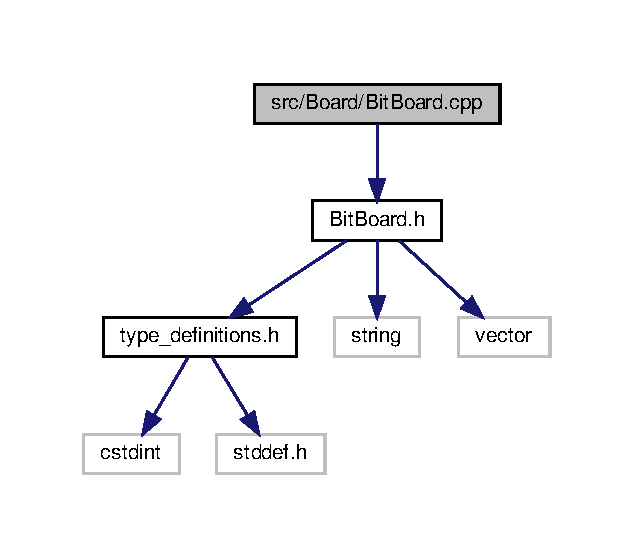
\includegraphics[width=304pt]{BitBoard_8cpp__incl}
\end{center}
\end{figure}
\subsection*{Functions}
\begin{DoxyCompactItemize}
\item 
\mbox{\Hypertarget{BitBoard_8cpp_aa64f191c32cc1987ad5bb3e7e2134b0a}\label{BitBoard_8cpp_aa64f191c32cc1987ad5bb3e7e2134b0a}} 
u64 {\bfseries perft} (\hyperlink{classBitBoard}{Bit\+Board} \&board, int depth)
\item 
\mbox{\Hypertarget{BitBoard_8cpp_a8013ad1288e56cd884d5d84119ba3b35}\label{BitBoard_8cpp_a8013ad1288e56cd884d5d84119ba3b35}} 
u64 {\bfseries perft\+\_\+leaf\+\_\+node\+\_\+optimization} (\hyperlink{classBitBoard}{Bit\+Board} \&board, int depth)
\end{DoxyCompactItemize}


\subsection{Detailed Description}
\begin{DoxyAuthor}{Author}
Harald Bjurulf (\href{mailto:haraldbjurulf@hotmail.com}{\tt haraldbjurulf@hotmail.\+com}) 
\end{DoxyAuthor}
\begin{DoxyVersion}{Version}
0.\+1 
\end{DoxyVersion}
\begin{DoxyDate}{Date}
2020-\/05-\/04
\end{DoxyDate}
\begin{DoxyCopyright}{Copyright}
Copyright (c) 2020 
\end{DoxyCopyright}

\hypertarget{BitBoard_8h}{}\section{src/\+Board/\+Bit\+Board.h File Reference}
\label{BitBoard_8h}\index{src/\+Board/\+Bit\+Board.\+h@{src/\+Board/\+Bit\+Board.\+h}}


Defines move and bitboard types.  


{\ttfamily \#include \char`\"{}type\+\_\+definitions.\+h\char`\"{}}\newline
{\ttfamily \#include $<$string$>$}\newline
{\ttfamily \#include $<$vector$>$}\newline
Include dependency graph for Bit\+Board.\+h\+:\nopagebreak
\begin{figure}[H]
\begin{center}
\leavevmode
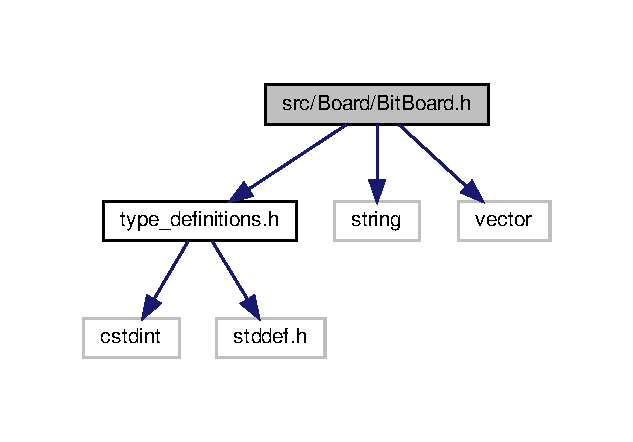
\includegraphics[width=304pt]{BitBoard_8h__incl}
\end{center}
\end{figure}
This graph shows which files directly or indirectly include this file\+:\nopagebreak
\begin{figure}[H]
\begin{center}
\leavevmode
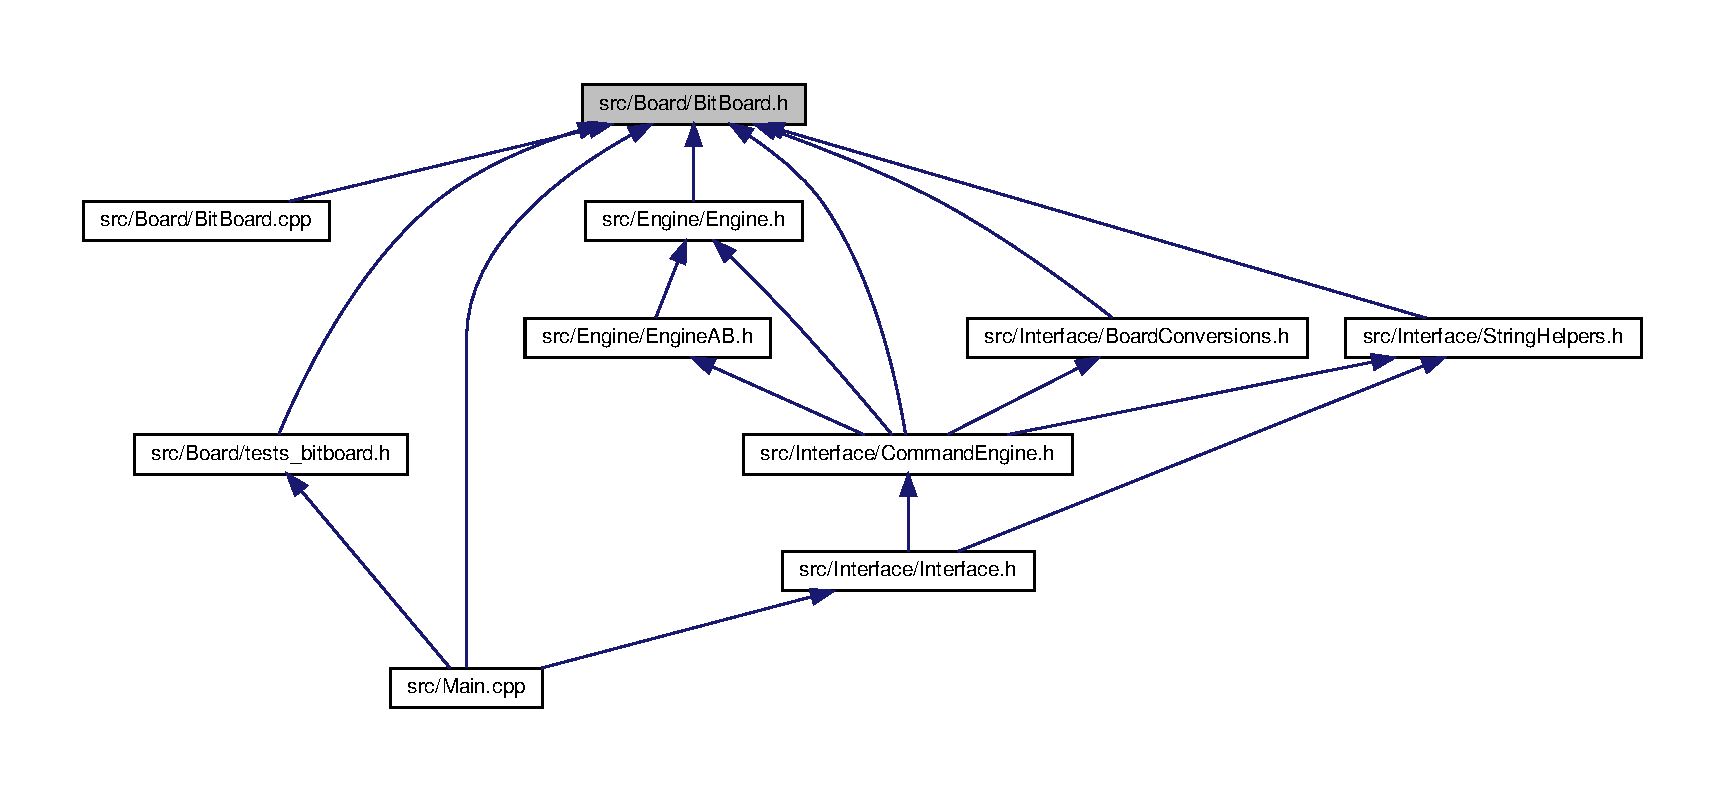
\includegraphics[width=350pt]{BitBoard_8h__dep__incl}
\end{center}
\end{figure}
\subsection*{Classes}
\begin{DoxyCompactItemize}
\item 
struct \hyperlink{structMove}{Move}
\begin{DoxyCompactList}\small\item\em represents a chess move and stores the necessary data to unmake the move \end{DoxyCompactList}\item 
struct \hyperlink{structBitBoardBase}{Bit\+Board\+Base}
\begin{DoxyCompactList}\small\item\em Wraps a vector to simplify move generation. \end{DoxyCompactList}\item 
struct \hyperlink{structMailBoardBase}{Mail\+Board\+Base}
\begin{DoxyCompactList}\small\item\em The basic data for a mail board. \end{DoxyCompactList}\item 
class \hyperlink{classBitBoard}{Bit\+Board}
\begin{DoxyCompactList}\small\item\em A complete chess board implementation including make and unmake move. \end{DoxyCompactList}\end{DoxyCompactItemize}
\subsection*{Functions}
\begin{DoxyCompactItemize}
\item 
\mbox{\Hypertarget{BitBoard_8h_aa64f191c32cc1987ad5bb3e7e2134b0a}\label{BitBoard_8h_aa64f191c32cc1987ad5bb3e7e2134b0a}} 
u64 {\bfseries perft} (\hyperlink{classBitBoard}{Bit\+Board} \&board, int depth)
\item 
\mbox{\Hypertarget{BitBoard_8h_a8013ad1288e56cd884d5d84119ba3b35}\label{BitBoard_8h_a8013ad1288e56cd884d5d84119ba3b35}} 
u64 {\bfseries perft\+\_\+leaf\+\_\+node\+\_\+optimization} (\hyperlink{classBitBoard}{Bit\+Board} \&board, int depth)
\end{DoxyCompactItemize}
\subsection*{Variables}
\begin{DoxyCompactItemize}
\item 
\mbox{\Hypertarget{BitBoard_8h_a082d99ab7bb470095769635c9feafd5e}\label{BitBoard_8h_a082d99ab7bb470095769635c9feafd5e}} 
const u64 {\bfseries O\+NE} = 1
\item 
\mbox{\Hypertarget{BitBoard_8h_a3905d1154dbccf9fcf170e609a07ee60}\label{BitBoard_8h_a3905d1154dbccf9fcf170e609a07ee60}} 
const u64 {\bfseries F\+U\+LL} = -\/1
\item 
\mbox{\Hypertarget{BitBoard_8h_afd955c0384c01306094bf3cb6eb09d97}\label{BitBoard_8h_afd955c0384c01306094bf3cb6eb09d97}} 
const u8 {\bfseries S\+I\+L\+E\+N\+T\+\_\+\+I\+N\+D\+EX} = 20
\item 
\mbox{\Hypertarget{BitBoard_8h_a77a6b63e996ff30ce48fac31132c87f5}\label{BitBoard_8h_a77a6b63e996ff30ce48fac31132c87f5}} 
const u64 {\bfseries S\+I\+L\+E\+N\+T\+\_\+\+M\+A\+SK} = ((u64)0b111111) $<$$<$ S\+I\+L\+E\+N\+T\+\_\+\+I\+N\+D\+EX
\item 
\mbox{\Hypertarget{BitBoard_8h_ac9940b8aad18b545371b306e80017eeb}\label{BitBoard_8h_ac9940b8aad18b545371b306e80017eeb}} 
const u8 {\bfseries U\+P\+G\+R\+A\+D\+E\+\_\+\+I\+N\+D\+EX} = 29
\item 
\mbox{\Hypertarget{BitBoard_8h_ae06b4c3840d806c6aeffa4d2838affe3}\label{BitBoard_8h_ae06b4c3840d806c6aeffa4d2838affe3}} 
const u64 {\bfseries U\+P\+G\+R\+A\+D\+E\+\_\+\+M\+A\+SK} = ((u64)0b111) $<$$<$ U\+P\+G\+R\+A\+D\+E\+\_\+\+I\+N\+D\+EX
\item 
\mbox{\Hypertarget{BitBoard_8h_a9cb4259930c2f16224c848d59f164f6b}\label{BitBoard_8h_a9cb4259930c2f16224c848d59f164f6b}} 
const u8 {\bfseries T\+A\+K\+E\+N\+\_\+\+I\+N\+D\+EX} = 26
\item 
\mbox{\Hypertarget{BitBoard_8h_a131c22cce427a88bdbf6be2308ef68fd}\label{BitBoard_8h_a131c22cce427a88bdbf6be2308ef68fd}} 
const u64 {\bfseries T\+A\+K\+E\+N\+\_\+\+M\+A\+SK} = ((u64)0b111) $<$$<$ T\+A\+K\+E\+N\+\_\+\+I\+N\+D\+EX
\item 
\mbox{\Hypertarget{BitBoard_8h_a6968fd882c739aa4657c7e245550099a}\label{BitBoard_8h_a6968fd882c739aa4657c7e245550099a}} 
const u8 {\bfseries F\+R\+O\+M\+\_\+\+I\+N\+D\+EX} = 0
\item 
\mbox{\Hypertarget{BitBoard_8h_af003e5d002d2908e81da3b5cff732820}\label{BitBoard_8h_af003e5d002d2908e81da3b5cff732820}} 
const u64 {\bfseries F\+R\+O\+M\+\_\+\+M\+A\+SK} = ((u64)0b111111) $<$$<$ F\+R\+O\+M\+\_\+\+I\+N\+D\+EX
\item 
\mbox{\Hypertarget{BitBoard_8h_ac42c8abbb4f015087216320b11e17943}\label{BitBoard_8h_ac42c8abbb4f015087216320b11e17943}} 
const u8 {\bfseries T\+O\+\_\+\+I\+N\+D\+EX} = 6
\item 
\mbox{\Hypertarget{BitBoard_8h_a2d2b50b2fe3b826a0a4f6aa58dd479ea}\label{BitBoard_8h_a2d2b50b2fe3b826a0a4f6aa58dd479ea}} 
const u64 {\bfseries T\+O\+\_\+\+M\+A\+SK} = ((u64)0b111111) $<$$<$ T\+O\+\_\+\+I\+N\+D\+EX
\item 
\mbox{\Hypertarget{BitBoard_8h_a974bdd847ff686fbc425777a754d04f5}\label{BitBoard_8h_a974bdd847ff686fbc425777a754d04f5}} 
const u8 {\bfseries E\+P\+\_\+\+I\+N\+D\+EX} = 12
\item 
\mbox{\Hypertarget{BitBoard_8h_a31faafc090860902f5d8a2b609b7f587}\label{BitBoard_8h_a31faafc090860902f5d8a2b609b7f587}} 
const u64 {\bfseries E\+P\+\_\+\+M\+A\+SK} = ((u64)0b1111) $<$$<$ E\+P\+\_\+\+I\+N\+D\+EX
\item 
\mbox{\Hypertarget{BitBoard_8h_abb63959b116de27fe1f4f41224eca5b8}\label{BitBoard_8h_abb63959b116de27fe1f4f41224eca5b8}} 
const u8 {\bfseries C\+A\+S\+T\+L\+I\+N\+G\+\_\+\+I\+N\+D\+EX} = 16
\item 
\mbox{\Hypertarget{BitBoard_8h_a7e0e9cfac6b3c53879cc7f028e52a905}\label{BitBoard_8h_a7e0e9cfac6b3c53879cc7f028e52a905}} 
const u64 {\bfseries C\+A\+S\+T\+L\+I\+N\+G\+\_\+\+M\+A\+SK} = ((u64)0b1111) $<$$<$ C\+A\+S\+T\+L\+I\+N\+G\+\_\+\+I\+N\+D\+EX
\end{DoxyCompactItemize}


\subsection{Detailed Description}
Defines move and bitboard types. 

\begin{DoxyAuthor}{Author}
Harald Bjurulf (\href{mailto:haraldbjurulf@hotmail.com}{\tt haraldbjurulf@hotmail.\+com}) 
\end{DoxyAuthor}
\begin{DoxyVersion}{Version}
0.\+1 
\end{DoxyVersion}
\begin{DoxyDate}{Date}
2020-\/05-\/04
\end{DoxyDate}
\begin{DoxyCopyright}{Copyright}
Copyright (c) 2020 
\end{DoxyCopyright}

\hypertarget{tests__bitboard_8h}{}\section{src/\+Board/tests\+\_\+bitboard.h File Reference}
\label{tests__bitboard_8h}\index{src/\+Board/tests\+\_\+bitboard.\+h@{src/\+Board/tests\+\_\+bitboard.\+h}}
{\ttfamily \#include $<$iostream$>$}\newline
{\ttfamily \#include \char`\"{}Bit\+Board.\+h\char`\"{}}\newline
{\ttfamily \#include $<$cstdint$>$}\newline
{\ttfamily \#include $<$cassert$>$}\newline
Include dependency graph for tests\+\_\+bitboard.\+h\+:\nopagebreak
\begin{figure}[H]
\begin{center}
\leavevmode
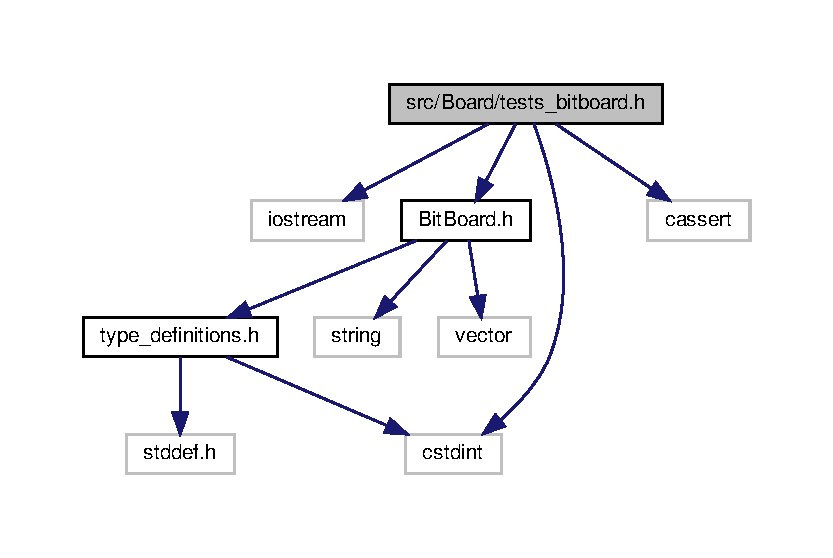
\includegraphics[width=350pt]{tests__bitboard_8h__incl}
\end{center}
\end{figure}
This graph shows which files directly or indirectly include this file\+:\nopagebreak
\begin{figure}[H]
\begin{center}
\leavevmode
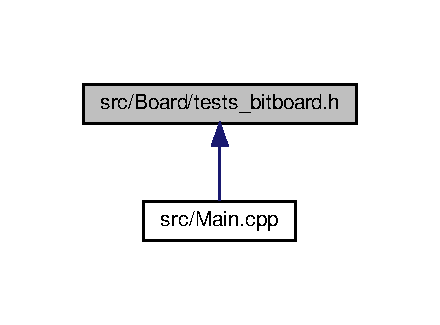
\includegraphics[width=211pt]{tests__bitboard_8h__dep__incl}
\end{center}
\end{figure}
\subsection*{Functions}
\begin{DoxyCompactItemize}
\item 
\mbox{\Hypertarget{tests__bitboard_8h_a4faa2b1253ebee4809759cae2fd23855}\label{tests__bitboard_8h_a4faa2b1253ebee4809759cae2fd23855}} 
void \hyperlink{tests__bitboard_8h_a4faa2b1253ebee4809759cae2fd23855}{test\+\_\+move} ()
\begin{DoxyCompactList}\small\item\em performs unit tests on the move type \end{DoxyCompactList}\item 
\mbox{\Hypertarget{tests__bitboard_8h_aca65d4b5f9c1ecf94272e0b466daf1b9}\label{tests__bitboard_8h_aca65d4b5f9c1ecf94272e0b466daf1b9}} 
void \hyperlink{tests__bitboard_8h_aca65d4b5f9c1ecf94272e0b466daf1b9}{test\+\_\+bitboard} ()
\begin{DoxyCompactList}\small\item\em Performs unit tests on the bitboard type. \end{DoxyCompactList}\item 
\mbox{\Hypertarget{tests__bitboard_8h_acb737e79cdc3f761b09dc11d12aa760d}\label{tests__bitboard_8h_acb737e79cdc3f761b09dc11d12aa760d}} 
int {\bfseries run\+\_\+tests\+\_\+bitboard} ()
\end{DoxyCompactItemize}


\subsection{Detailed Description}
\begin{DoxyAuthor}{Author}
Harald Bjurulf (\href{mailto:haraldbjurulf@hotmail.com}{\tt haraldbjurulf@hotmail.\+com}) 
\end{DoxyAuthor}
\begin{DoxyVersion}{Version}
0.\+1 
\end{DoxyVersion}
\begin{DoxyDate}{Date}
2020-\/05-\/04
\end{DoxyDate}
\begin{DoxyCopyright}{Copyright}
Copyright (c) 2020 
\end{DoxyCopyright}

\hypertarget{Engine_8h}{}\section{src/\+Engine/\+Engine.h File Reference}
\label{Engine_8h}\index{src/\+Engine/\+Engine.\+h@{src/\+Engine/\+Engine.\+h}}


Contains the \hyperlink{classEngine}{Engine} base class.  


{\ttfamily \#include $<$vector$>$}\newline
{\ttfamily \#include $<$iostream$>$}\newline
{\ttfamily \#include \char`\"{}../\+Board/\+Bit\+Board.\+h\char`\"{}}\newline
Include dependency graph for Engine.\+h\+:\nopagebreak
\begin{figure}[H]
\begin{center}
\leavevmode
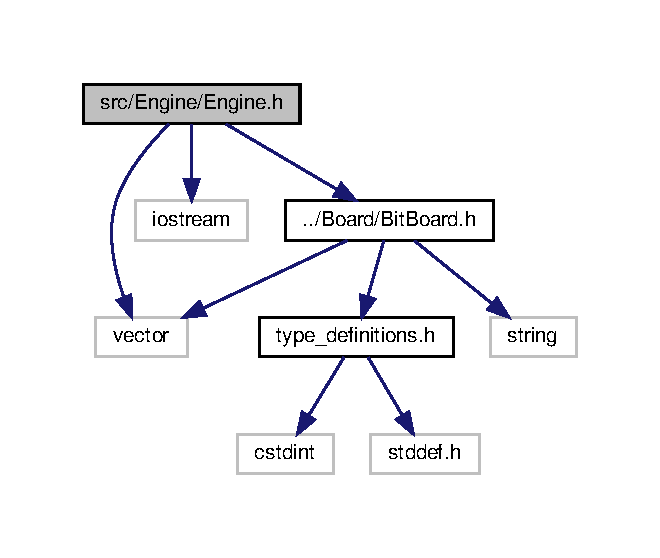
\includegraphics[width=317pt]{Engine_8h__incl}
\end{center}
\end{figure}
This graph shows which files directly or indirectly include this file\+:\nopagebreak
\begin{figure}[H]
\begin{center}
\leavevmode
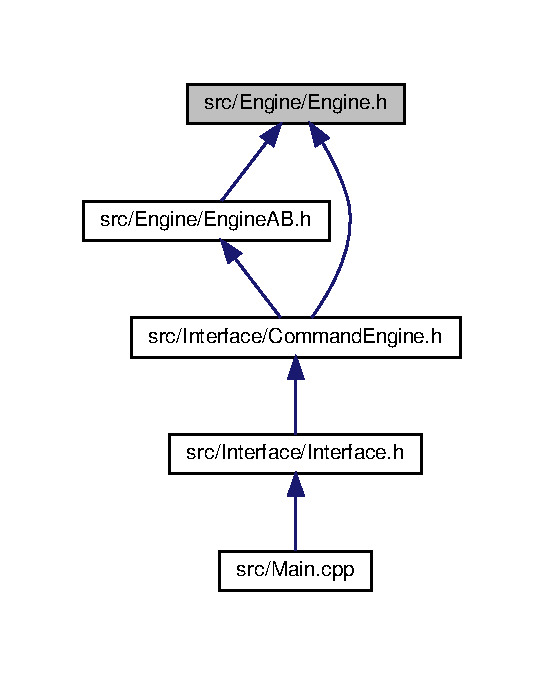
\includegraphics[width=261pt]{Engine_8h__dep__incl}
\end{center}
\end{figure}
\subsection*{Classes}
\begin{DoxyCompactItemize}
\item 
class \hyperlink{classEngine}{Engine}
\begin{DoxyCompactList}\small\item\em Base Chess \hyperlink{classEngine}{Engine} class, defines common variables and functions needed for children. \end{DoxyCompactList}\end{DoxyCompactItemize}


\subsection{Detailed Description}
Contains the \hyperlink{classEngine}{Engine} base class. 

\begin{DoxyAuthor}{Author}
William Sandström and Harald Bjurulf 
\end{DoxyAuthor}
\begin{DoxyVersion}{Version}
0.\+1 
\end{DoxyVersion}
\begin{DoxyDate}{Date}
2020-\/05-\/05
\end{DoxyDate}
\begin{DoxyCopyright}{Copyright}
Copyright (c) 2020 
\end{DoxyCopyright}

\hypertarget{EngineAB_8h}{}\section{src/\+Engine/\+Engine\+AB.h File Reference}
\label{EngineAB_8h}\index{src/\+Engine/\+Engine\+A\+B.\+h@{src/\+Engine/\+Engine\+A\+B.\+h}}


Contains the class \hyperlink{classEngineAlphaBeta}{Engine\+Alpha\+Beta}.  


{\ttfamily \#include $<$iostream$>$}\newline
{\ttfamily \#include \char`\"{}Engine.\+h\char`\"{}}\newline
Include dependency graph for Engine\+A\+B.\+h\+:\nopagebreak
\begin{figure}[H]
\begin{center}
\leavevmode
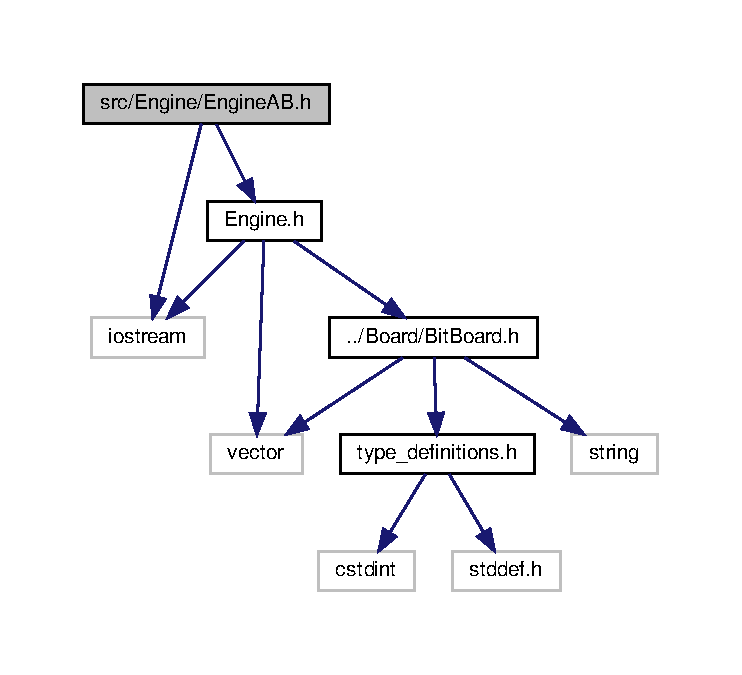
\includegraphics[width=350pt]{EngineAB_8h__incl}
\end{center}
\end{figure}
This graph shows which files directly or indirectly include this file\+:\nopagebreak
\begin{figure}[H]
\begin{center}
\leavevmode
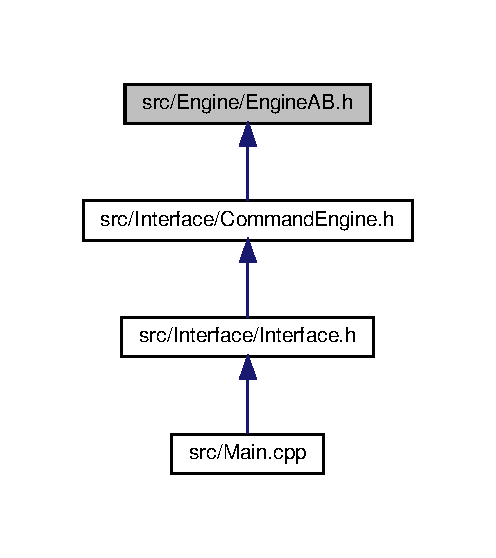
\includegraphics[width=238pt]{EngineAB_8h__dep__incl}
\end{center}
\end{figure}
\subsection*{Classes}
\begin{DoxyCompactItemize}
\item 
class \hyperlink{classEngineAlphaBeta}{Engine\+Alpha\+Beta}
\begin{DoxyCompactList}\small\item\em Alpha Beta Chess \hyperlink{classEngine}{Engine} class. Inherits from base class \hyperlink{classEngine}{Engine}. \end{DoxyCompactList}\end{DoxyCompactItemize}


\subsection{Detailed Description}
Contains the class \hyperlink{classEngineAlphaBeta}{Engine\+Alpha\+Beta}. 

\begin{DoxyAuthor}{Author}
William Sandström and Harald Bjurulf 
\end{DoxyAuthor}
\begin{DoxyVersion}{Version}
0.\+1 
\end{DoxyVersion}
\begin{DoxyDate}{Date}
2020-\/05-\/05
\end{DoxyDate}
\begin{DoxyCopyright}{Copyright}
Copyright (c) 2020 
\end{DoxyCopyright}

\hypertarget{BoardConversions_8h}{}\section{src/\+Interface/\+Board\+Conversions.h File Reference}
\label{BoardConversions_8h}\index{src/\+Interface/\+Board\+Conversions.\+h@{src/\+Interface/\+Board\+Conversions.\+h}}


This file contains the static class \hyperlink{classBoardConversions}{Board\+Conversions}.  


{\ttfamily \#include $<$string$>$}\newline
{\ttfamily \#include \char`\"{}../\+Board/\+Bit\+Board.\+h\char`\"{}}\newline
Include dependency graph for Board\+Conversions.\+h\+:\nopagebreak
\begin{figure}[H]
\begin{center}
\leavevmode
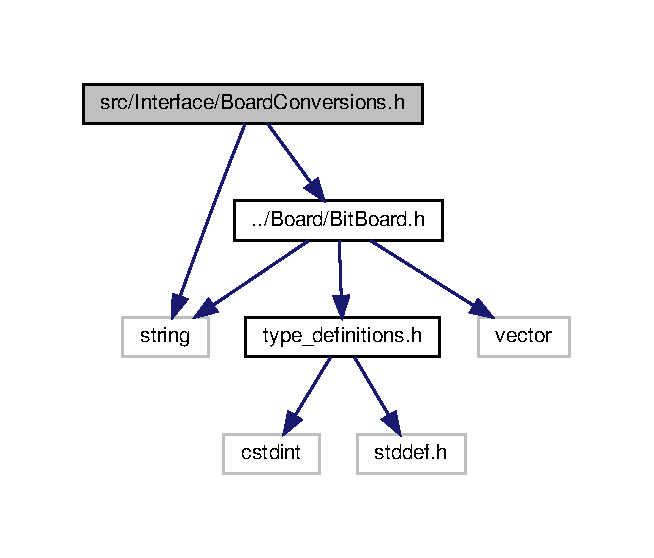
\includegraphics[width=314pt]{BoardConversions_8h__incl}
\end{center}
\end{figure}
This graph shows which files directly or indirectly include this file\+:\nopagebreak
\begin{figure}[H]
\begin{center}
\leavevmode
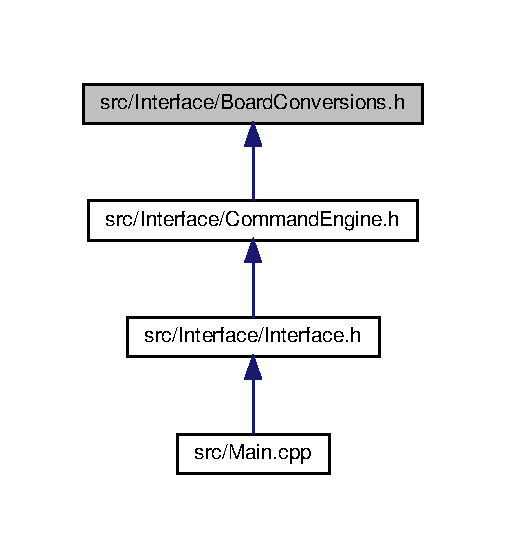
\includegraphics[width=243pt]{BoardConversions_8h__dep__incl}
\end{center}
\end{figure}
\subsection*{Classes}
\begin{DoxyCompactItemize}
\item 
class \hyperlink{classBoardConversions}{Board\+Conversions}
\begin{DoxyCompactList}\small\item\em This is a static helper class which is used for various Board state conversions and also other types of conversions which are needed. \end{DoxyCompactList}\end{DoxyCompactItemize}


\subsection{Detailed Description}
This file contains the static class \hyperlink{classBoardConversions}{Board\+Conversions}. 

\begin{DoxyAuthor}{Author}
William Sandström and Harald Bjurulf 
\end{DoxyAuthor}
\begin{DoxyVersion}{Version}
0.\+1 
\end{DoxyVersion}
\begin{DoxyDate}{Date}
2020-\/05-\/05
\end{DoxyDate}
\begin{DoxyCopyright}{Copyright}
Copyright (c) 2020 
\end{DoxyCopyright}

\hypertarget{CommandEngine_8h}{}\section{src/\+Interface/\+Command\+Engine.h File Reference}
\label{CommandEngine_8h}\index{src/\+Interface/\+Command\+Engine.\+h@{src/\+Interface/\+Command\+Engine.\+h}}


This file contains the \hyperlink{classCommandEngine}{Command\+Engine} class.  


{\ttfamily \#include $<$iostream$>$}\newline
{\ttfamily \#include $<$thread$>$}\newline
{\ttfamily \#include $<$atomic$>$}\newline
{\ttfamily \#include $<$chrono$>$}\newline
{\ttfamily \#include $<$vector$>$}\newline
{\ttfamily \#include \char`\"{}String\+Helpers.\+h\char`\"{}}\newline
{\ttfamily \#include \char`\"{}Board\+Conversions.\+h\char`\"{}}\newline
{\ttfamily \#include \char`\"{}../\+Engine/\+Engine\+A\+B.\+h\char`\"{}}\newline
{\ttfamily \#include \char`\"{}../\+Engine/\+Engine.\+h\char`\"{}}\newline
{\ttfamily \#include \char`\"{}../\+Board/\+Bit\+Board.\+h\char`\"{}}\newline
Include dependency graph for Command\+Engine.\+h\+:\nopagebreak
\begin{figure}[H]
\begin{center}
\leavevmode
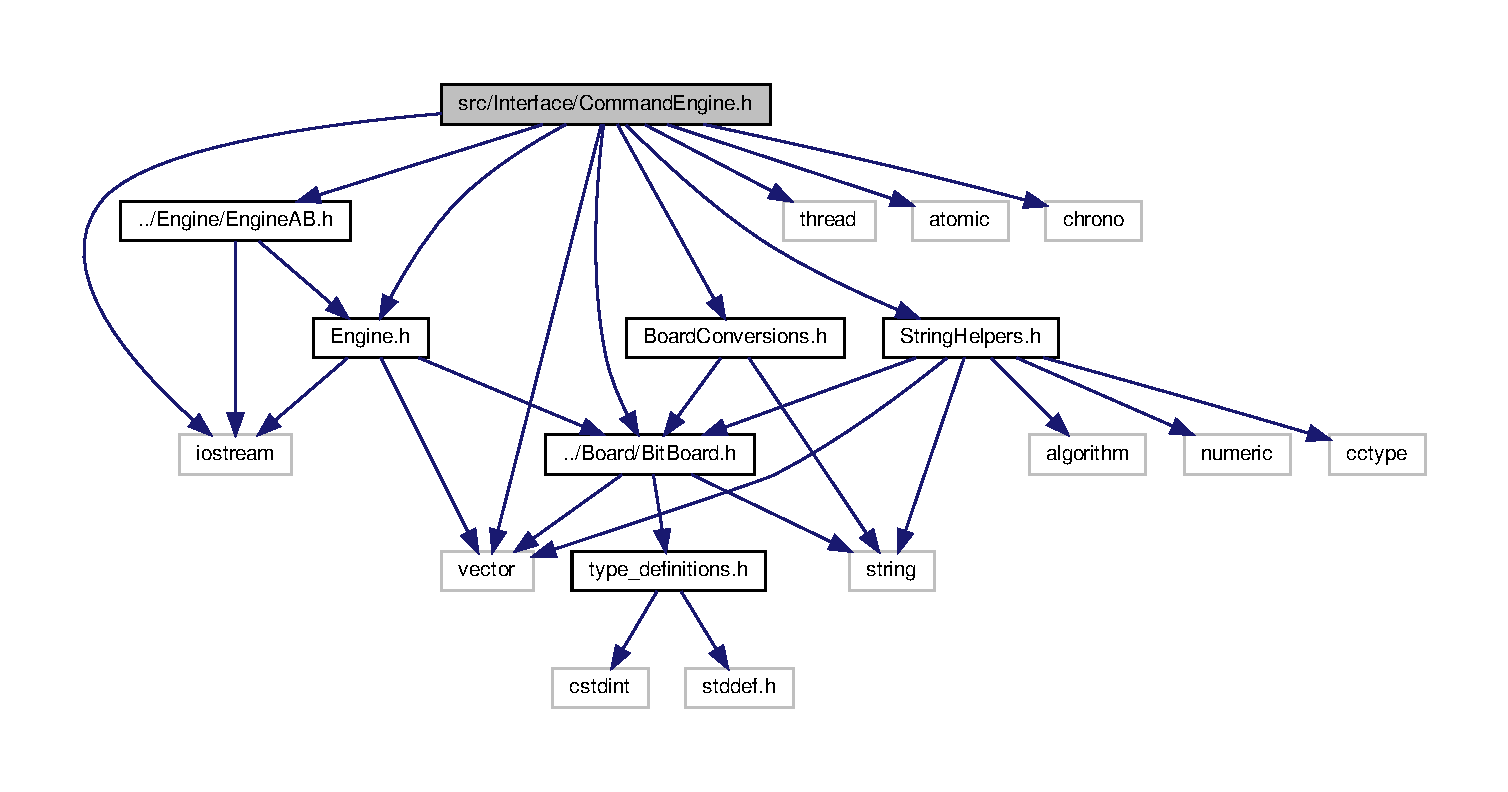
\includegraphics[width=350pt]{CommandEngine_8h__incl}
\end{center}
\end{figure}
This graph shows which files directly or indirectly include this file\+:\nopagebreak
\begin{figure}[H]
\begin{center}
\leavevmode
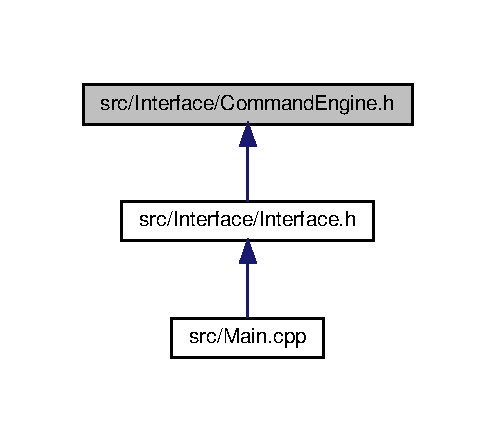
\includegraphics[width=238pt]{CommandEngine_8h__dep__incl}
\end{center}
\end{figure}
\subsection*{Classes}
\begin{DoxyCompactItemize}
\item 
class \hyperlink{classCommandEngine}{Command\+Engine}
\begin{DoxyCompactList}\small\item\em This class contains functions related to executing various commands sent from the \hyperlink{classInterface}{Interface}. \end{DoxyCompactList}\end{DoxyCompactItemize}
\subsection*{Variables}
\begin{DoxyCompactItemize}
\item 
\mbox{\Hypertarget{CommandEngine_8h_a1fb188b65b89f6581f50397dca40d0ab}\label{CommandEngine_8h_a1fb188b65b89f6581f50397dca40d0ab}} 
const std\+::string {\bfseries E\+N\+G\+I\+N\+E\+\_\+\+N\+A\+ME} = \char`\"{}Magnificence2\char`\"{}
\item 
\mbox{\Hypertarget{CommandEngine_8h_a98054aebdb48537787d82f070f03387e}\label{CommandEngine_8h_a98054aebdb48537787d82f070f03387e}} 
const std\+::string {\bfseries A\+U\+T\+H\+O\+R\+\_\+\+N\+A\+ME} = \char`\"{}Prog\+Boys\char`\"{}
\item 
const std\+::string {\bfseries H\+E\+L\+P\+\_\+\+S\+T\+R\+I\+NG}
\end{DoxyCompactItemize}


\subsection{Detailed Description}
This file contains the \hyperlink{classCommandEngine}{Command\+Engine} class. 

\begin{DoxyAuthor}{Author}
William Sandström and Harald Bjurulf 
\end{DoxyAuthor}
\begin{DoxyVersion}{Version}
0.\+1 
\end{DoxyVersion}
\begin{DoxyDate}{Date}
2020-\/05-\/05
\end{DoxyDate}
\begin{DoxyCopyright}{Copyright}
Copyright (c) 2020 
\end{DoxyCopyright}


\subsection{Variable Documentation}
\mbox{\Hypertarget{CommandEngine_8h_a9eac5a48402885e5270a5d998d47ace3}\label{CommandEngine_8h_a9eac5a48402885e5270a5d998d47ace3}} 
\index{Command\+Engine.\+h@{Command\+Engine.\+h}!H\+E\+L\+P\+\_\+\+S\+T\+R\+I\+NG@{H\+E\+L\+P\+\_\+\+S\+T\+R\+I\+NG}}
\index{H\+E\+L\+P\+\_\+\+S\+T\+R\+I\+NG@{H\+E\+L\+P\+\_\+\+S\+T\+R\+I\+NG}!Command\+Engine.\+h@{Command\+Engine.\+h}}
\subsubsection{\texorpdfstring{H\+E\+L\+P\+\_\+\+S\+T\+R\+I\+NG}{HELP\_STRING}}
{\footnotesize\ttfamily const std\+::string H\+E\+L\+P\+\_\+\+S\+T\+R\+I\+NG}

{\bfseries Initial value\+:}
\begin{DoxyCode}
= 
    \textcolor{stringliteral}{"Command list: \(\backslash\)n"}
    \textcolor{stringliteral}{"help                   Display a list of commands\(\backslash\)n"}
    \textcolor{stringliteral}{"quit                   Exit the program\(\backslash\)n"}
    \textcolor{stringliteral}{"display                Display the board in the console \(\backslash\)n"}
    \textcolor{stringliteral}{"go         [depth]     Search with the current Engine\(\backslash\)n"}
    \textcolor{stringliteral}{"perft      <depth>     Calculate perft for current position\(\backslash\)n"}
    \textcolor{stringliteral}{"divide     <depth>     Perft score per each legal move of current position.\(\backslash\)n"}
    \textcolor{stringliteral}{"fen                    Display the fen string for the current board\(\backslash\)n"}
    \textcolor{stringliteral}{"setboard   <fen>       Set the board to a fen string\(\backslash\)n"}
    \textcolor{stringliteral}{"move       <move>      Peform an algebraic move\(\backslash\)n"}
    \textcolor{stringliteral}{"moves                  List legal moves\(\backslash\)n"}
    \textcolor{stringliteral}{"selfplay               Play a game between two Engines\(\backslash\)n"}
    \textcolor{stringliteral}{"uci                    Enter UCI mode\(\backslash\)n"}
\end{DoxyCode}

\hypertarget{Interface_8h}{}\section{src/\+Interface/\+Interface.h File Reference}
\label{Interface_8h}\index{src/\+Interface/\+Interface.\+h@{src/\+Interface/\+Interface.\+h}}


This file contains the \hyperlink{classInterface}{Interface} class.  


{\ttfamily \#include $<$iostream$>$}\newline
{\ttfamily \#include $<$thread$>$}\newline
{\ttfamily \#include $<$sstream$>$}\newline
{\ttfamily \#include $<$string$>$}\newline
{\ttfamily \#include $<$unordered\+\_\+map$>$}\newline
{\ttfamily \#include \char`\"{}Command\+Engine.\+h\char`\"{}}\newline
{\ttfamily \#include \char`\"{}String\+Helpers.\+h\char`\"{}}\newline
Include dependency graph for Interface.\+h\+:\nopagebreak
\begin{figure}[H]
\begin{center}
\leavevmode
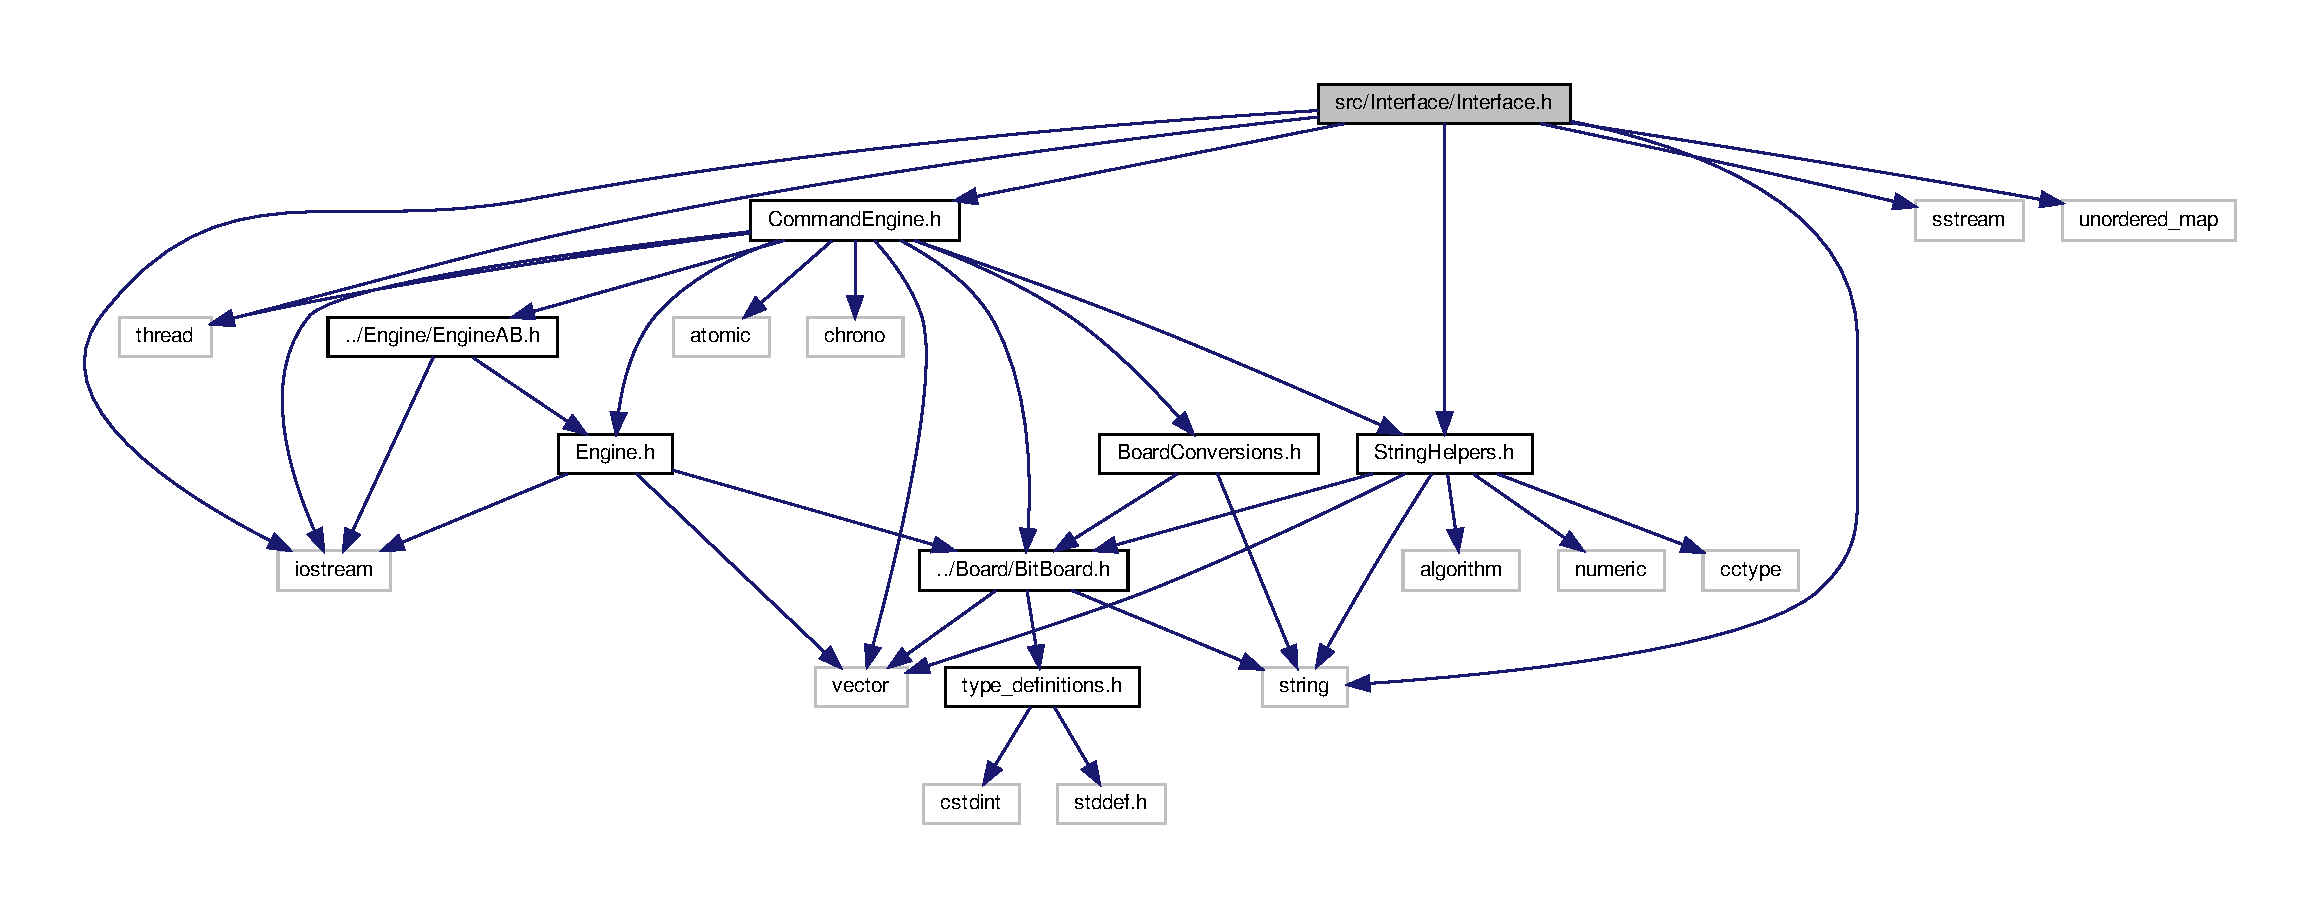
\includegraphics[width=350pt]{Interface_8h__incl}
\end{center}
\end{figure}
This graph shows which files directly or indirectly include this file\+:\nopagebreak
\begin{figure}[H]
\begin{center}
\leavevmode
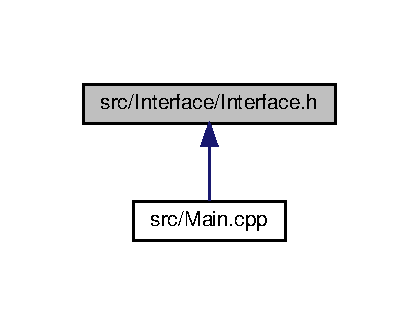
\includegraphics[width=201pt]{Interface_8h__dep__incl}
\end{center}
\end{figure}
\subsection*{Classes}
\begin{DoxyCompactItemize}
\item 
class \hyperlink{classInterface}{Interface}
\begin{DoxyCompactList}\small\item\em The main \hyperlink{classInterface}{Interface} class for the program. It controls the main command loop, reads input and executes commands by calling functions in \hyperlink{classCommandEngine}{Command\+Engine}. \end{DoxyCompactList}\end{DoxyCompactItemize}
\subsection*{Variables}
\begin{DoxyCompactItemize}
\item 
const std\+::string {\bfseries W\+E\+L\+C\+O\+M\+E\+\_\+\+M\+E\+S\+S\+A\+GE}
\end{DoxyCompactItemize}


\subsection{Detailed Description}
This file contains the \hyperlink{classInterface}{Interface} class. 

\begin{DoxyAuthor}{Author}
William Sandström and Harald Bjurulf 
\end{DoxyAuthor}
\begin{DoxyVersion}{Version}
0.\+1 
\end{DoxyVersion}
\begin{DoxyDate}{Date}
2020-\/05-\/05
\end{DoxyDate}
\begin{DoxyCopyright}{Copyright}
Copyright (c) 2020 
\end{DoxyCopyright}


\subsection{Variable Documentation}
\mbox{\Hypertarget{Interface_8h_abef0057416aa7d589821f3a7bf3f8047}\label{Interface_8h_abef0057416aa7d589821f3a7bf3f8047}} 
\index{Interface.\+h@{Interface.\+h}!W\+E\+L\+C\+O\+M\+E\+\_\+\+M\+E\+S\+S\+A\+GE@{W\+E\+L\+C\+O\+M\+E\+\_\+\+M\+E\+S\+S\+A\+GE}}
\index{W\+E\+L\+C\+O\+M\+E\+\_\+\+M\+E\+S\+S\+A\+GE@{W\+E\+L\+C\+O\+M\+E\+\_\+\+M\+E\+S\+S\+A\+GE}!Interface.\+h@{Interface.\+h}}
\subsubsection{\texorpdfstring{W\+E\+L\+C\+O\+M\+E\+\_\+\+M\+E\+S\+S\+A\+GE}{WELCOME\_MESSAGE}}
{\footnotesize\ttfamily const std\+::string W\+E\+L\+C\+O\+M\+E\+\_\+\+M\+E\+S\+S\+A\+GE}

{\bfseries Initial value\+:}
\begin{DoxyCode}
= 
    \textcolor{stringliteral}{"--------------------------------\(\backslash\)n"}
    \textcolor{stringliteral}{"Magnificence 2 Development Build\(\backslash\)n"}
    \textcolor{stringliteral}{"--------------------------------\(\backslash\)n"}
\end{DoxyCode}

\hypertarget{StringHelpers_8h}{}\section{src/\+Interface/\+String\+Helpers.h File Reference}
\label{StringHelpers_8h}\index{src/\+Interface/\+String\+Helpers.\+h@{src/\+Interface/\+String\+Helpers.\+h}}


This file contains the static \hyperlink{classStringHelpers}{String\+Helpers} class and the \hyperlink{structStringArguments}{String\+Arguments} class.  


{\ttfamily \#include $<$string$>$}\newline
{\ttfamily \#include $<$vector$>$}\newline
{\ttfamily \#include $<$algorithm$>$}\newline
{\ttfamily \#include $<$numeric$>$}\newline
{\ttfamily \#include $<$cctype$>$}\newline
{\ttfamily \#include \char`\"{}../\+Board/\+Bit\+Board.\+h\char`\"{}}\newline
Include dependency graph for String\+Helpers.\+h\+:\nopagebreak
\begin{figure}[H]
\begin{center}
\leavevmode
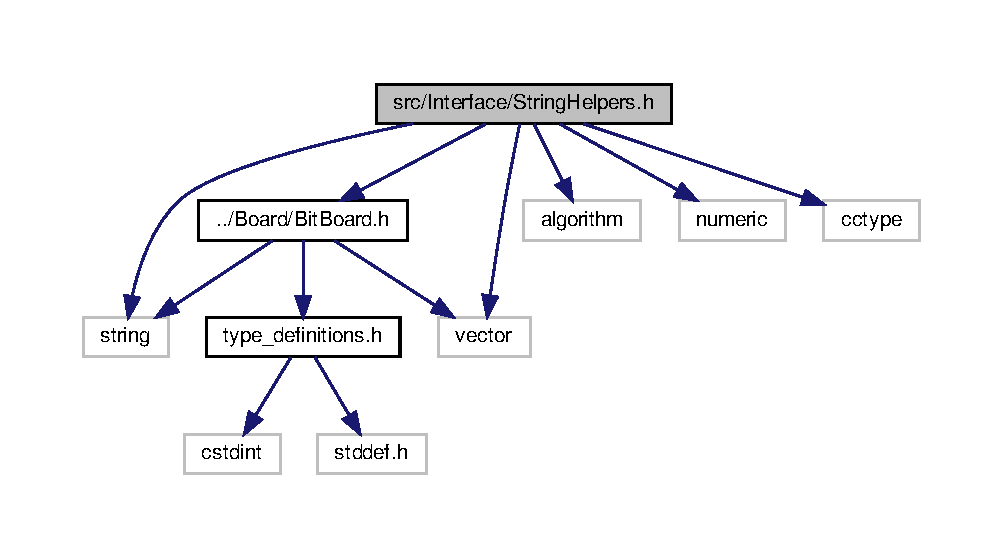
\includegraphics[width=350pt]{StringHelpers_8h__incl}
\end{center}
\end{figure}
This graph shows which files directly or indirectly include this file\+:\nopagebreak
\begin{figure}[H]
\begin{center}
\leavevmode
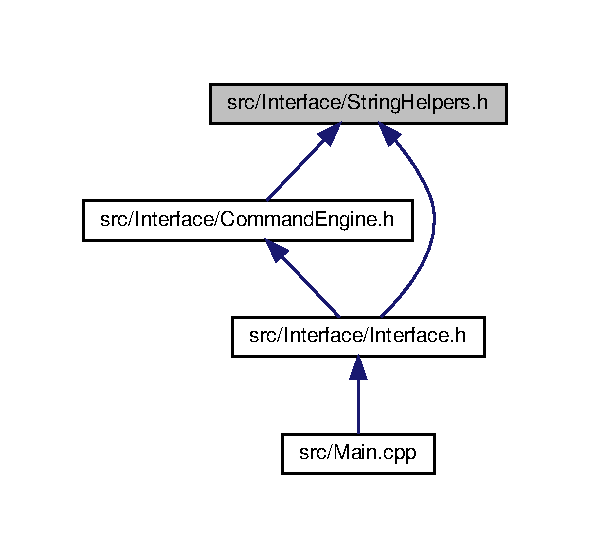
\includegraphics[width=283pt]{StringHelpers_8h__dep__incl}
\end{center}
\end{figure}
\subsection*{Classes}
\begin{DoxyCompactItemize}
\item 
class \hyperlink{classStringHelpers}{String\+Helpers}
\begin{DoxyCompactList}\small\item\em A static helper class which is used for various common string tasks, such as string splitting. \end{DoxyCompactList}\item 
struct \hyperlink{structStringArguments}{String\+Arguments}
\begin{DoxyCompactList}\small\item\em A class which is used to represents command inputs by splitting them up in parts for easier access. \end{DoxyCompactList}\end{DoxyCompactItemize}


\subsection{Detailed Description}
This file contains the static \hyperlink{classStringHelpers}{String\+Helpers} class and the \hyperlink{structStringArguments}{String\+Arguments} class. 

\begin{DoxyAuthor}{Author}
William Sandström and Harald Bjurulf 
\end{DoxyAuthor}
\begin{DoxyVersion}{Version}
0.\+1 
\end{DoxyVersion}
\begin{DoxyDate}{Date}
2020-\/05-\/05
\end{DoxyDate}
\begin{DoxyCopyright}{Copyright}
Copyright (c) 2020 
\end{DoxyCopyright}

\hypertarget{Main_8cpp}{}\section{src/\+Main.cpp File Reference}
\label{Main_8cpp}\index{src/\+Main.\+cpp@{src/\+Main.\+cpp}}


Entry point for application.  


{\ttfamily \#include $<$iostream$>$}\newline
{\ttfamily \#include \char`\"{}Board/\+Bit\+Board.\+h\char`\"{}}\newline
{\ttfamily \#include \char`\"{}Board/tests\+\_\+bitboard.\+h\char`\"{}}\newline
{\ttfamily \#include \char`\"{}Interface/\+Interface.\+h\char`\"{}}\newline
Include dependency graph for Main.\+cpp\+:\nopagebreak
\begin{figure}[H]
\begin{center}
\leavevmode
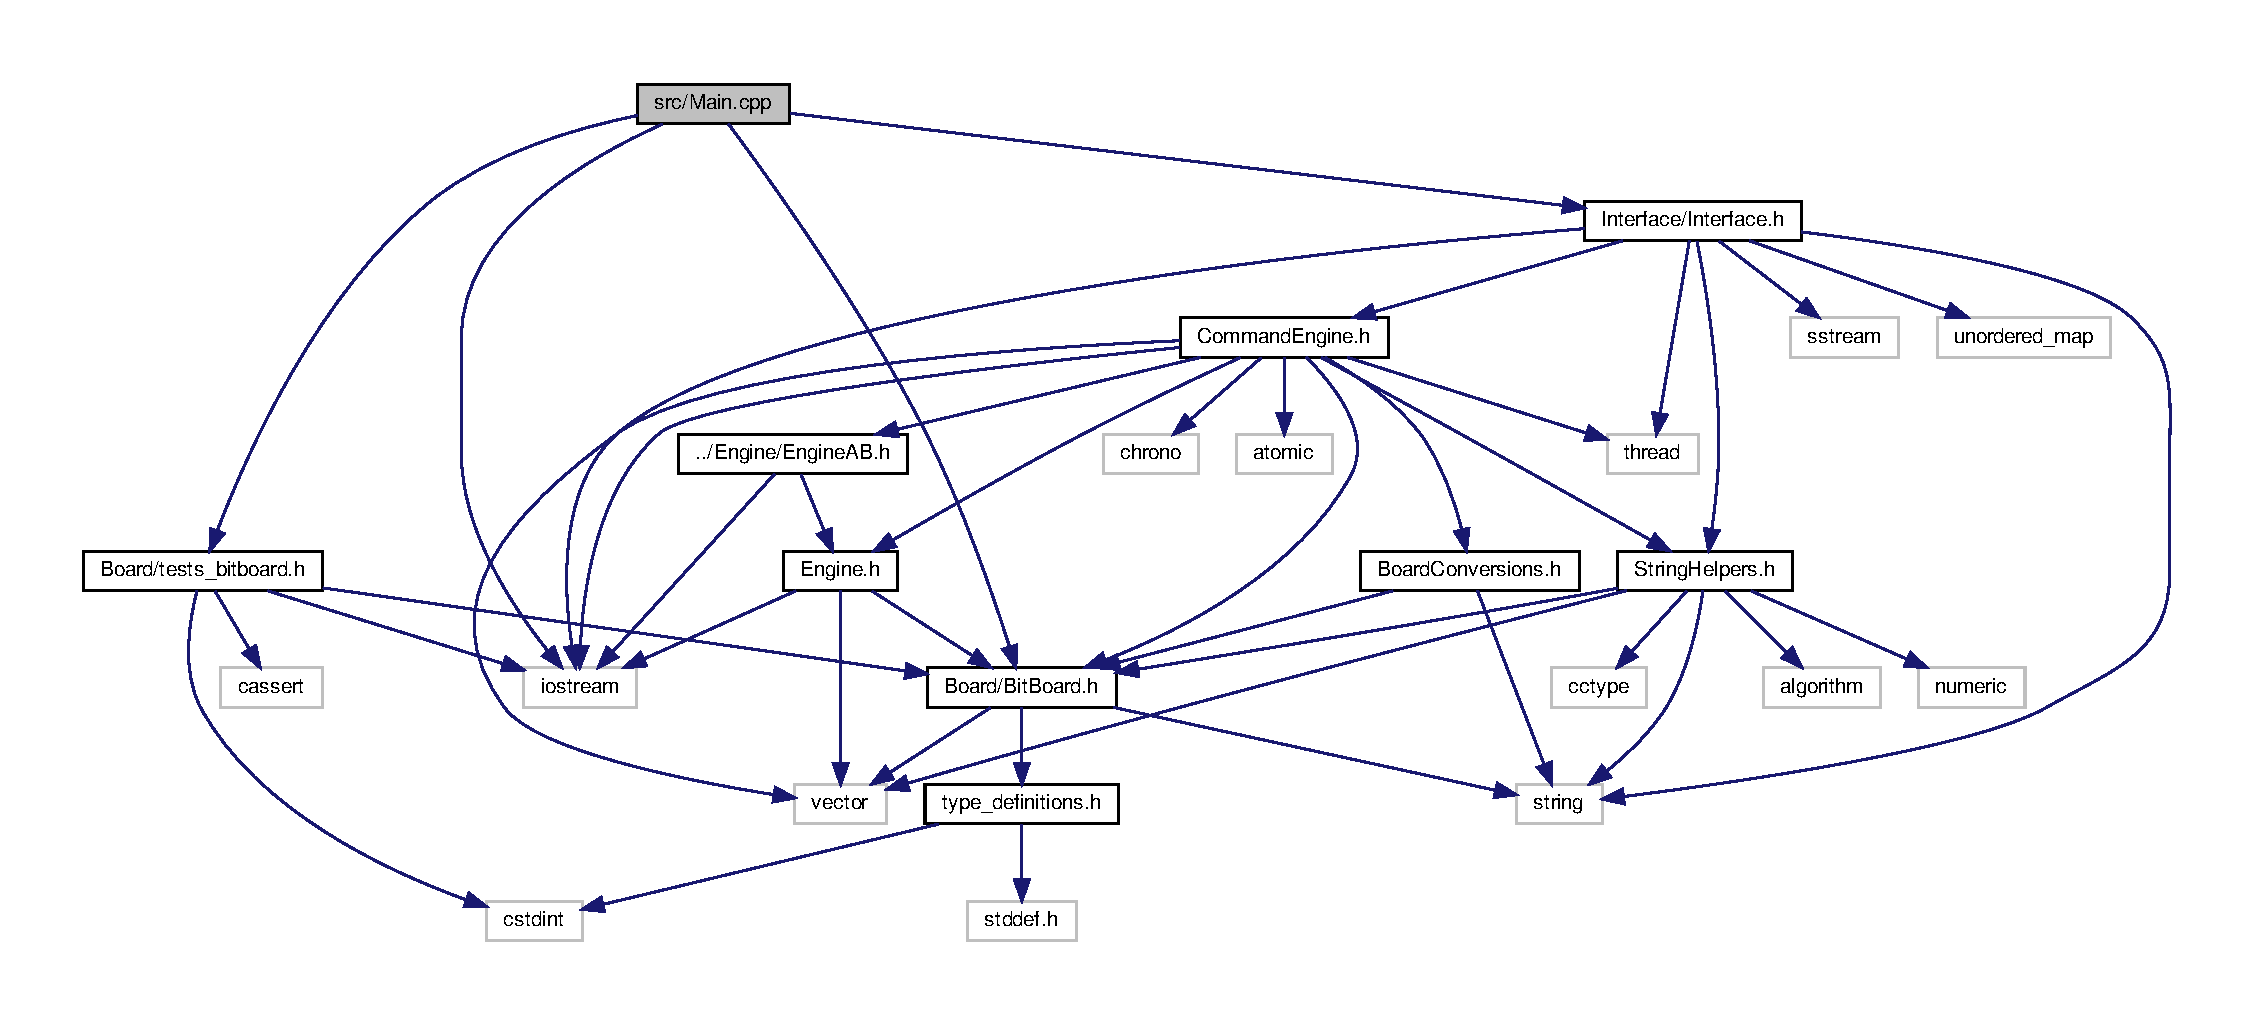
\includegraphics[width=350pt]{Main_8cpp__incl}
\end{center}
\end{figure}
\subsection*{Macros}
\begin{DoxyCompactItemize}
\item 
\mbox{\Hypertarget{Main_8cpp_ad72dbcf6d0153db1b8d8a58001feed83}\label{Main_8cpp_ad72dbcf6d0153db1b8d8a58001feed83}} 
\#define {\bfseries D\+E\+B\+UG}~1
\end{DoxyCompactItemize}
\subsection*{Functions}
\begin{DoxyCompactItemize}
\item 
\mbox{\Hypertarget{Main_8cpp_ae66f6b31b5ad750f1fe042a706a4e3d4}\label{Main_8cpp_ae66f6b31b5ad750f1fe042a706a4e3d4}} 
int \hyperlink{Main_8cpp_ae66f6b31b5ad750f1fe042a706a4e3d4}{main} ()
\begin{DoxyCompactList}\small\item\em Runs tests if in D\+E\+B\+UG and executes the main command loop by creating the \hyperlink{classInterface}{Interface} class. \end{DoxyCompactList}\end{DoxyCompactItemize}


\subsection{Detailed Description}
Entry point for application. 

\begin{DoxyAuthor}{Author}
William Sandström 
\end{DoxyAuthor}
\begin{DoxyVersion}{Version}
0.\+1 
\end{DoxyVersion}
\begin{DoxyDate}{Date}
2020-\/05-\/05
\end{DoxyDate}
\begin{DoxyCopyright}{Copyright}
Copyright (c) 2020 
\end{DoxyCopyright}

%--- End generated contents ---

% Index
\backmatter
\newpage
\phantomsection
\clearemptydoublepage
\addcontentsline{toc}{chapter}{Index}
\printindex

\end{document}
